%==============================================================================
%  main_cn.tex — 中文对照稿（非投稿件）
%
%  用途：给院内评审与中文读者看的对照稿，内容与 main_applsci_mdpicls.tex 一致。
%  它不是投稿文件，所以不套 MDPI 的版面家具（那是 Applied Sciences 的排版，
%  中文稿套上去只会不伦不类）；用干净的单栏中文学术版式。
%
%  编译：xelatex main_cn.tex（两遍）
%  本机字体：AR PL UMing CN（正文，宋体类）、WenQuanYi Zen Hei（粗体与标题）、
%           AR PL UKai CN（楷体，用于强调）。为什么不用 Noto 见下方字体设置处的
%           注释。装配记录见 ../LOOP_STATE.md。
%
%  图：按要求不翻译 —— 图内文字保持英文，图题译成中文。
%  图与表的代码是从英文稿逐字搬过来的，只有题注是中文；
%  `verify_cn.py` 断言两边非题注部分完全一致，防止两份稿子的图表悄悄漂移。
%==============================================================================
\documentclass[11pt,a4paper]{article}

\usepackage{xeCJK}
% 字体按中文惯例配：宋体正文、黑体加粗与标题、楷体强调。
% 注意不要用 Noto Sans CJK SC —— 它是 .ttc 字体集合，本机 TeX Live 2013 的
% xdvipdfmx 无法从集合中取表，编译看起来 0 error，驱动却以 "sfnt: table not
% found" 失败并删掉 PDF。已逐个字体实测，见 ../LOOP_STATE.md。
\setCJKmainfont[BoldFont={WenQuanYi Zen Hei},
                ItalicFont={AR PL UKai CN}]{AR PL UMing CN}
\setCJKsansfont[BoldFont={WenQuanYi Zen Hei}]{WenQuanYi Micro Hei}
\setCJKmonofont{WenQuanYi Micro Hei Mono}
\xeCJKsetup{CJKmath=true}

\usepackage{mathptmx}          % 西文与英文稿一致，用 Times
\usepackage[T1]{fontenc}
\usepackage{amsmath,amssymb,textcomp}
\usepackage[a4paper,left=2.6cm,right=2.6cm,top=2.8cm,bottom=2.6cm]{geometry}
\linespread{1.28}
\usepackage{graphicx}
\usepackage{array,booktabs,longtable,colortbl}
\usepackage{xcolor}
\usepackage{caption}
\usepackage{enumitem}
\usepackage{float}
% mdpi.cls 的通栏表格用 \begin{adjustwidth}{-\extralength}{0cm} 向页边扩展。
% 中文稿是普通 article 类，没有这两样东西。这里补上等价定义，
% 而不是在搬运时把它们删掉 —— 删掉就破坏了"图表代码与英文稿逐字一致"
% 这条断言。
\usepackage{changepage}
% \extralength 不能取 0：MDPI 的宽表是故意伸出正文块的，取 0 等于取消了这个设计，
% 两张七列表会各溢出约 50pt。mdpi.cls 原值是 4.61cm（它的正文块只有 13.4cm，
% 右侧还留着行号栏）；中文版面 15.8cm 放不下那么多扩展，按本页面重算取 2.0cm。
\newlength{\extralength}\setlength{\extralength}{2.0cm}
\usepackage{tikz}
\usetikzlibrary{shapes.geometric,arrows.meta,positioning,fit,backgrounds,calc}
% pgfplots 设置必须与英文稿一致，否则同一份图代码渲染结果会不同：
% compat 版本影响默认行为，groupplots 是图 2 的 (a)(b) 双面板所必需的。
\usepackage{pgfplots}
\pgfplotsset{compat=1.16}
\usepgfplotslibrary{groupplots}
\usepackage[colorlinks=true,allcolors=blue]{hyperref}
\urlstyle{same}

%--- 与英文稿同一套色（Okabe-Ito，色觉障碍下可分辨）
\definecolor{okVermillion}{HTML}{D55E00}
\definecolor{okOrange}{HTML}{E69F00}
\definecolor{okYellow}{HTML}{F0E442}
\definecolor{okGreen}{HTML}{009E73}
\definecolor{okBlue}{HTML}{0072B2}
\definecolor{okSky}{HTML}{56B4E9}
\definecolor{okPurple}{HTML}{CC79A7}
\definecolor{okGold}{HTML}{8C6D31}

\newcommand{\PH}[1]{{\color{red}\textbf{[#1]}}}
% 未译段落用它标出来，红色、显眼，且可被 verify_cn.py 计数：
% 只要还剩一处，这份稿子就不算译完。
\newcommand{\todocn}[1]{{\color{red}\textbf{【待译：#1】}}}
\newcommand{\doilink}[1]{\begingroup\urlstyle{same}\url{#1}\endgroup}
\newcolumntype{L}[1]{>{\raggedright\arraybackslash}p{#1}}
\newcolumntype{C}[1]{>{\centering\arraybackslash}p{#1}}
\newcommand{\tnote}[1]{\textsuperscript{#1}}
% 以下三个宏被搬入的图表用到，定义与英文稿逐字相同 —— 搬运图表代码时，
% 它所依赖的宏也必须一起过来，否则编译会在离成因很远的地方报错。
\newcommand{\panel}[2]{{\small(\textbf{#1})~#2}}
\newcommand{\tabfoot}[1]{\par\vspace{2pt}\begingroup\raggedright\footnotesize
  \noindent #1\par\endgroup}
\newcommand{\tnotedef}[1]{\textsuperscript{#1}\,}

%--- 中文版式：标题用黑体，图题在下、表题在上
\usepackage{titlesec}
\titleformat{\section}{\sffamily\bfseries\large}{\thesection}{0.6em}{}
\titleformat{\subsection}{\sffamily\bfseries\normalsize}{\thesubsection}{0.6em}{}
\titleformat{\subsubsection}{\sffamily\bfseries\normalsize}{\thesubsubsection}{0.6em}{}
\titlespacing{\section}{0pt}{14pt plus 2pt minus 2pt}{6pt}
\titlespacing{\subsection}{0pt}{11pt plus 2pt minus 2pt}{4pt}
\captionsetup{font=small,labelfont={sf,bf},labelsep=quad,
              justification=raggedright,singlelinecheck=false}
\captionsetup[table]{position=above,skip=4pt}
\captionsetup[figure]{position=below,skip=6pt}
\renewcommand{\figurename}{图}
\renewcommand{\tablename}{表}
\renewcommand{\refname}{参考文献}
\setlength{\parindent}{2em}

\begin{document}

%==============================================================================
%  前置件
%==============================================================================
\begin{center}
{\sffamily\bfseries\LARGE 以元数据为基的大语言模型：\\[2pt]
把医院统计需求转成临床数据仓库查询\par}

\vspace{10pt}
{\normalsize 李世凯\par}
\vspace{4pt}
{\small 四川大学华西医院\ 信息与数据管理部，成都\ 610041\par}
\vspace{2pt}
{\small 通信作者邮箱：\PH{author@example.edu}\qquad 电话：\PH{+86 ...}\par}
\end{center}

\vspace{6pt}
\noindent\fbox{\begin{minipage}{\dimexpr\linewidth-2\fboxsep-2\fboxrule}
\small\textbf{应用场景}\quad 本框架把临床科室提交的自由文本统计需求转成可执行、
带血缘的 SQL，在医院临床数据仓库上运行，使医院管理所依赖的科室绩效、质控与
上报指标在给出数字的同时一并给出它是按什么口径统计的，而不是把口径留在查询里。
系统本地部署，患者数据不出院；遇到口径有争议时，把它退回指标责任人，
而不是自己悄悄定一个。
\end{minipage}}

\vspace{10pt}
\noindent{\sffamily\bfseries 摘要}\quad
医院报表依赖的统计口径——一个病例按哪个时间点计入、哪个标志位定义一个指标——
是各院自定的，没有跨院通用词表，因此临床科室的自由文本需求在到达数据库之前，
总要先经过一名数据工程师。本文把这类需求转成三层临床数据仓库上可执行的
Presto SQL：生成过程以元数据知识库为基，每条候选查询都经过语法、字段、口径与
结果四道校验。在 30 项报表任务的 398 个业务术语上，映射准确率为 52.3\%，
生产环境规则匹配器为 32.9\%（$p<0.001$）。一项覆盖 24 项任务、8 个模型、
5 种提示策略的因子实验产生 960 次生成，其中 791 次产出 SQL，274 次含字段或
口径错误。本地部署的 qwen2.5:7b 有效 SQL 率最高，71.7\%（95\% CI 63.0--79.0），
gpt-4o 为 60.8\%——原因是它幻觉更少，而不是它生成得更多。口径错误是最大的
一类错误，占 34.7\%；这类错误产出的是一条能跑通、但数字是错的查询，
通用的 schema-linking 错误分类里没有这个类别。由于这类错误会悄悄改变上报指标的
分母，本文明确给出：已测得的可靠性支持哪些绩效管理与质控用途，以及哪些残余风险
仍然留在医院这一侧。

\vspace{6pt}
\noindent{\sffamily\bfseries 关键词}\quad text-to-SQL；大语言模型；临床数据仓库；
幻觉；元数据；统计口径；医院信息系统；检索增强生成；医院管理；绩效测量

\vspace{4pt}
\noindent{\footnotesize 英文标题：Metadata-Grounded Large Language Models for
Converting Hospital Statistical Requests into Clinical Data Warehouse Queries。
本文为英文投稿件 \texttt{main\_applsci\_mdpicls.tex} 的中文对照稿，
所有数值与英文稿同源。\par}

\vspace{10pt}
\hrule
\vspace{10pt}

%==============================================================================
\section{引言}
%==============================================================================
医院运营报表是质量控制、绩效管理与临床研究的基础，但它在数据获取这一环上
长期存在瓶颈。在本院，临床科室、质量管理办公室与研究者提交的统计需求，
都排队交给一支人数不多的数据工程团队处理；2023--2024 年间，
\PH{XX：等待超过五个工作日的占比}\% 的需求等待首个结果超过五个工作日，
\PH{XX：交付后仍需再澄清一轮的占比}\% 在交付后仍需至少一轮口径澄清。
这些延迟推后了管理决策；对研究类需求而言，则拉长了研究周期、抬高了成本，
最终限制了医院对自己已经拥有的数据发问的频次。

延迟不是全部代价。医院管理是靠"可比"的指标运转的：绩效考核里科室与科室比，
质控里本月与上月比，上报里本院与同行比。而比较之所以携带信息，前提是每个数字
背后的统计口径相同；当每张报表都是手写的，这个口径就只存在于查询里，
而不在任何医院可以查阅的目录中。两位分析师在不同季度被要求统计"急诊手术量"，
可能筛的是不同的标志位，而且各自都能给出说得通的理由；管理层随后读到的"趋势"，
其实是"谁写的查询"的产物。这种失效是安静的——按错口径写出的查询照样能跑，
照样返回一个看起来合理的数字。因此，一条报表流水线欠医院的不只是那个数字，
还有它是按什么口径统计出来的，并且要以指标责任人能够复核的形式给出；
而当口径确实存在争议时，还要有一种"把争议说出来"的办法，而不是默默选一个。

临床数据仓库（clinical data warehouse，CDW）的存在正是为了缓解这一压力。
本院的仓库采用三层设计——数据湖（DL）、数据中心（DC）与主数据仓库（MDR）——
把手术麻醉、输血、检验、病理与计费系统标准化为面向主题的模型，
通过 Presto 查询 \cite{presto2019}。这消除了大部分关联复杂度；
在国际上，承担同一角色的是 OMOP 这类共享通用数据模型 \cite{ohdsi2015}，
不过本院的报表是针对院内自定指标定义的，而非基于共享词表。然而，
把一条自由文本统计需求转成仓库查询依然困难，因为需求编码的是\emph{统计口径}
而不是数据结构。入室时间、手术结束时间、出院时间与申请时间在计数上并不等价；
"择期手术""非计划再次手术""并发症"都是院内自定的定义，
其计数对象、时间口径与筛选条件必须先被还原出来，SQL 才写得下去。

用自然语言直接查询结构化临床数据，此前沿三条线展开。text-to-SQL 这条线从
序列到序列的语义解析器，发展到 schema linking、约束解码与分解式上下文学习架构，
并在公开基准上评测 \cite{zhong2017,yu2018,wang2020,scholak2021,pourreza2023,bird2023,dailsql2024,macsql2024}；
它通过面向电子病历的数据集、在其上训练的生成模型，以及对不可答问题给出弃权
即予奖励的可靠性导向评测任务，被带入临床场景
\cite{treqs2020,medts2021,ehrsql2024,ragepi2024,rag2step2025}。
本文使用的评测框架沿用自上述其中一项研究——它把临床试验入排标准转成
OMOP 通用数据模型查询，并在八个模型、五种提示策略下刻画幻觉模式
\cite{lee2025}：八模型的云端/本地对比、五种提示策略、开发集与验证集的划分、
幻觉类别的五级严重度排序，都是他们的；我们沿用这些，是为了让本文的数字能与
他们的并排阅读。真正不同的是被查询的对象。他们的口径是针对共享通用数据模型的
入排规则，一个概念要么在词表里、要么不在；我们的是院内自定的统计口径，
字段存在、查询能跑、数字却仍然是错的。这一差别正是本文分类中 Category B
所度量的东西，而它在共享词表的场景里没有对应物。另有一项工作在
MIMIC-III 与 TREQS 上评测了六个较新的模型，报告了同样的准确率--成本张力，
并把检索增强与术语整合列为值得一试的对策 \cite{tankovic2025}；
本文所述系统两者都已实现，并量化了各自的贡献。
另一条线把自由文本的入排标准转成可执行的队列查询，从基于规则与解析器的系统
到模块化查询生成器 \cite{c2q2019,trialpath2021,leafai2023}。
把元数据增强与任务分解用于临床注册库查询并报告了显著提升的工作也已出现
\cite{metaclin2025}。尽管有这些进展，从统计需求自动生成仓库查询仍面临一个
关键的可靠性挑战：大模型经常给出并不存在的列名与表名；而对医院报表更为致命的是，
它会指派一个看似合理但错误的统计口径——这种失效产出的是一条能执行的查询
和一个错的数字。

近期研究表明，大模型虽然在自然语言理解上很强，但在把领域术语映射到受控词表与
库表结构时错误率相当高，且该错误率随模型与提示大幅波动
\cite{halluc2024,ragstruct2024,chang2024}。这一可靠性缺口构成了临床落地的
实质障碍，因为口径映射错了不会"大声"失败——它悄悄改变了一个可能要上报监管部门的
质量指标的分母。此外，医院部署还多了一条基准研究不会遇到的约束：
患者数据不得离开医院，因此云端模型只能用于去标识化的元数据，
而云端与本地模型的取舍会实质影响准确率与成本。在这一约束下的系统性模型对比
目前仍然很少。

本研究从两个方面回应上述问题。第一，我们给出一套端到端的自动化系统，
把自由文本的医院统计需求转成符合本院三层 CDW 的 Presto SQL，
并用四川大学华西医院的真实患者数据加以验证。第二，我们在 SynHDW（仓库的
去标识化合成镜像）上对 8 个大模型（云端与本地各半）的幻觉模式做了系统评测，
分析模型选择与提示工程如何影响可靠性。结果显示，大模型可以把查询生成从数天
压到数分钟，但 20\%--47\% 的幻觉率说明模型选择与校验策略必须谨慎。
出乎意料的是，模型规模并不必然与表现正相关：较小的本地模型在有效 SQL 生成上
胜过了更大的商业模型。通过量化这些取舍、并为不同报表场景找出较优的
模型--提示组合，本工作推进了面向医院数据运营的可信、低成本 AI 系统。

%==============================================================================
\section{材料与方法}
%==============================================================================

\subsection{研究设计}
本研究分两阶段进行：先开发并验证一套把医院统计需求自动转成三层 CDW 上
Presto SQL 的系统，再对大模型的幻觉模式做系统分析。两阶段合成一条工作流，
使得在真实报表场景下既能做功能验证，也能做可靠性评估。

\subsection{数据来源与研究对象}

\subsubsection{统计需求数据集}
我们从四川大学华西医院的报表工单系统中提取统计需求（数据访问日期
2026 年 7 月 27 日），只保留那些已经关单、且带有工程师撰写并经口径确认的
参考 SQL 的工单。共使用两个数据集：（1）开发集；（2）验证集。

开发集含 30 项报表任务（手术麻醉、输血、检验三个领域各 10 项），
仅用于构建元数据字典与优化提示。我们从这些任务中抽取出 412 个唯一业务术语，
用于大模型与院内规则匹配器（RBFM）的映射方法对比。

验证集按前 24 个月的需求频次选出 7 项高频报表任务（RPT-001 各科室月度择期
手术量；RPT-002 非计划再次手术率；RPT-003 麻醉后监护室（PACU）通过量与
延迟离室率；RPT-004 月度输血量与输血反应率；RPT-005 检验危急值通报及时率；
RPT-006 手术部位感染监测分母；RPT-007 日间手术占手术总量比例），
用于系统的整体评估。

\subsubsection{临床数据基础设施}
真实数据验证使用四川大学华西医院的生产 CDW：一个基于 Presto 的三层平台
（DL/DC/MDR），整合 26 个源系统。该数据集含 1\,620\,000 名唯一患者，
临床记录跨 2016 年 3 月至 2025 年 2 月，通过 398 张标准化表、
逾 13\,000 个字段对外提供。所有表都带逻辑删除标志，多院区表还带机构码；
两者在每一条生成的查询中都必须被筛选。研究方案经四川大学华西医院
伦理委员会批准（批号 \PH{XXXX-XXXX}）。

\subsubsection{用于幻觉分析的合成数据}
为系统评估幻觉模式，我们使用合成医院数据仓库（Synthetic Hospital Data
Warehouse，SynHDW）1.0 版（生成种子 20251118）——生产仓库的去标识化合成镜像，
含 112\,680 名合成患者，带 2019 至 2023 年的就诊、手术、输血与检验记录。
该数据集的元数据覆盖有限（约 1680 个字段，生产环境为 13\,000 余个），
恰好成为一个理想的试验台：可以观察模型在字段与口径映射遇到困难时的幻觉行为。

\subsection{统计口径到 SQL 的转换流水线}
流水线由三个模块把自由文本的统计需求转成符合 Presto 的 SQL。预处理分三个阶段：
切分——把需求拆成逐条口径，同时保留布尔逻辑与分组层次；过滤——去掉不可查询的成分，
如排版要求、截止时间与叙述性理由；简化——统一时间表达并压缩 token 数，
但不改变统计语义。信息抽取模块从预处理后的文本中识别七类结构化成分
（业务术语、元数据系统［仓库结构、指标口径字典、历史 SQL、例外规则］、字段标识、
取值、属性、时间、否定），随后按检索增强生成的做法，用大模型把每个业务术语映射到
仓库标准化字段与统计口径 \cite{lewis2020,finardi2024}。候选表与字段由稀疏--稠密
混合方案召回，即 BM25 \cite{bm252009} 与 transformer 句向量
\cite{sbert2019,bert2019} 相结合；这一召回步骤承担的是 schema linking 的角色，
近期工作把它刻画为上下文感知的双向检索，其核心张力在召回与精确之间——
链接过于激进就会把无关的结构成分一并纳入 \cite{schemalink2025,rslsql2024}。
SQL 生成模块通过迭代精化与优化产出符合 Presto 的查询，并为每条查询附带一份
字段血缘记录。各模块之间以结构化 JSON 交换数据，以保证全流水线的互操作性。
图~\ref{fig:arch} 给出流水线整体；补充材料的图 S1 把每个模块展开为其组成步骤，
并标明模块之间的接口。

%%CNFLOAT-BEGIN:fig:arch%%
\begin{figure}[H]
\centering
\vspace{2pt}

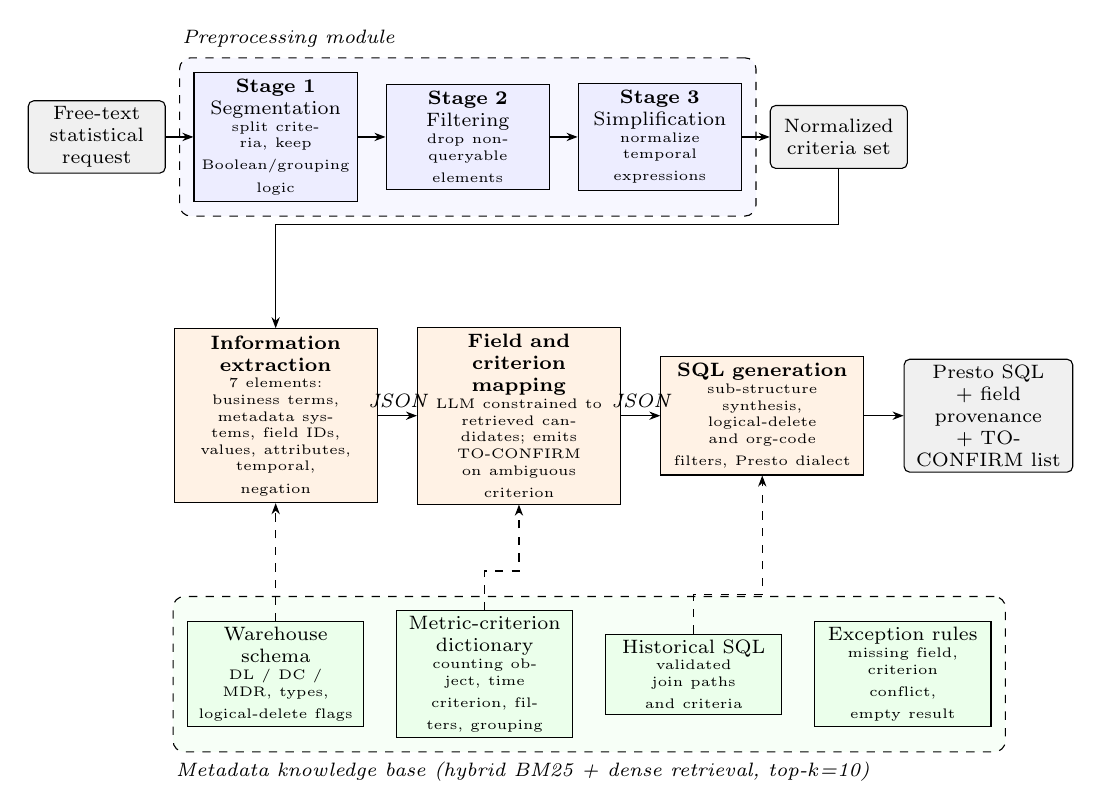
\begin{tikzpicture}[
  font=\scriptsize,
  node distance=3.2mm and 3.5mm,
  io/.style   ={draw,rounded corners=2pt,fill=gray!12,align=center,
                text width=16mm,minimum height=8mm,inner sep=2pt},
  st/.style   ={draw,fill=blue!7,align=center,text width=19mm,
                minimum height=11mm,inner sep=2.5pt},
  mod/.style  ={draw,fill=orange!10,align=center,text width=23mm,
                minimum height=12mm,inner sep=2.5pt},
  kb/.style   ={draw,fill=green!8,align=center,text width=21mm,
                minimum height=7mm,inner sep=2pt},
  lbl/.style  ={font=\scriptsize\itshape,inner sep=1pt},
  >={Stealth[length=4pt]}]

% ---------- Row 1 : preprocessing ----------
\node[io]  (req) {Free-text\\statistical request};
\node[st, right=of req] (s1) {\textbf{Stage 1}\\Segmentation\\{\tiny split criteria, keep\\Boolean/grouping logic}};
\node[st, right=of s1]  (s2) {\textbf{Stage 2}\\Filtering\\{\tiny drop non-queryable\\elements}};
\node[st, right=of s2]  (s3) {\textbf{Stage 3}\\Simplification\\{\tiny normalize temporal\\expressions}};
\node[io, right=of s3]  (norm) {Normalized\\criteria set};

\draw[->] (req)--(s1); \draw[->] (s1)--(s2); \draw[->] (s2)--(s3); \draw[->] (s3)--(norm);

\begin{scope}[on background layer]
\node[draw,dashed,rounded corners,fill=blue!3,inner sep=5pt,fit=(s1)(s2)(s3)] (pre) {};
\end{scope}
\node[lbl,anchor=south west,yshift=0.8mm] at (pre.north west) {Preprocessing module};

% ---------- Row 2 : information extraction ----------
\node[mod, below=16mm of s1.south, anchor=north, text width=24mm] (ie)
  {\textbf{Information extraction}\\{\tiny 7 elements: business terms,\\metadata systems, field IDs,\\values, attributes, temporal,\\negation}};
\node[mod, right=5mm of ie, text width=24mm] (map)
  {\textbf{Field and criterion}\\\textbf{mapping}\\{\tiny LLM constrained to\\retrieved candidates; emits\\TO-CONFIRM on ambiguous\\criterion}};
\node[mod, right=5mm of map, text width=24mm] (gen)
  {\textbf{SQL generation}\\{\tiny sub-structure synthesis,\\logical-delete and org-code\\filters, Presto dialect}};
\node[io, right=5mm of gen, text width=20mm] (out)
  {Presto SQL\\+ field provenance\\+ TO-CONFIRM list};

\draw[->] (norm.south) -- ++(0,-7mm) -| (ie.north);
\draw[->] (ie)--(map); \draw[->] (map)--(gen); \draw[->] (gen)--(out);

% ---------- Row 3 : knowledge base ----------
\node[kb, below=15mm of ie.south, anchor=north] (kb1) {Warehouse schema\\{\tiny DL / DC / MDR, types,\\logical-delete flags}};
\node[kb, right=4mm of kb1] (kb2) {Metric-criterion dictionary\\{\tiny counting object, time\\criterion, filters, grouping}};
\node[kb, right=4mm of kb2] (kb3) {Historical SQL\\{\tiny validated join paths\\and criteria}};
\node[kb, right=4mm of kb3] (kb4) {Exception rules\\{\tiny missing field, criterion\\conflict, empty result}};

\begin{scope}[on background layer]
\node[draw,dashed,rounded corners,fill=green!3,inner sep=5pt,
      fit=(kb1)(kb2)(kb3)(kb4)] (kbx) {};
\end{scope}
\node[lbl,anchor=north west,yshift=-0.8mm] at (kbx.south west)
  {Metadata knowledge base (hybrid BM25 + dense retrieval, top-$k$=10)};

\draw[->,dashed] (kb1.north) -- ++(0,5mm) -| (ie.south);
\draw[->,dashed] (kb2.north) -- ++(0,5mm) -| (map.south);
\draw[->,dashed] (kb3.north) -- ++(0,5mm) -| (gen.south);

% ---------- JSON annotation ----------
\node[lbl,above=0.6mm] at ($(ie.east)!0.5!(map.west)$)  {JSON};
\node[lbl,above=0.6mm] at ($(map.east)!0.5!(gen.west)$) {JSON};

\end{tikzpicture}
\caption{转换流水线的结构。一条自由文本的医院统计需求依次经过三阶段预处理、信息抽取、字段与口径映射、SQL 生成，最终在三层临床数据仓库（CDW）上产出与 Presto 兼容的结构化查询语言（SQL），同时给出字段血缘记录与全部 TO-CONFIRM 条目。实线箭头表示模块间的数据流；虚线箭头表示各模块读取元数据知识库的哪一部分。DC：数据中心；DL：数据湖；JSON：JavaScript 对象表示法；LLM：大语言模型；MDR：主数据仓库。}
\label{fig:arch}
\end{figure}
%%CNFLOAT-END:fig:arch%%

\subsection{大模型配置}
我们通过 API 使用 gpt-4o（版本 gpt-4o-2024-08-06），并以 vLLM 在本地部署
qwen2.5:7b-instruct，各任务的提示策略经迭代精化后确定。对需求切分、口径分类
这类直接的任务采用零样本提示，以尽量降低 token 用量与推理成本；
对字段与口径映射、SQL 生成这类复杂任务，则用精选示例的少样本提示以提升表现。
所有提示都包含三项明确要求：遵循 Presto 方言、必须筛选逻辑删除与机构码、
以及错误处理。所有模型均采用确定性解码（temperature 0，top-$p$ 1）。
没有任何患者级数据被发往云端；云端模型只接收去标识化的元数据与合成取值。
完整的提示模板见补充材料表 S2。

\subsection{对比评测框架}

\subsubsection{业务术语映射评估}
映射准确率在 30 项任务的开发集（手术麻醉、输血、检验）上评估，
该集覆盖了较宽的院内术语范围。我们把大模型与本院元数据门户中现役的
规则字段匹配器（rule-based field matcher，RBFM）作对比。RBFM 是院内自研工具、
无法在别处重跑，因此我们另外报告一个外部可复现的参照：对每个业务术语，
在列名与注释上用 BM25 取分值最高的那一个仓库字段，不用同义词表、
也不含语义成分。大模型做的是带上下文的自然语言理解，而 RBFM 用的是
字符串规范化、基于 Levenshtein 距离的相似度打分，以及一份人工整理的同义词表
来找候选字段。实验中 RBFM 按其生产配置运行，对每个输入术语取相似度分值最高的字段。
各任务的相关业务术语从需求文本中抽出，同时交给大模型与 RBFM 映射。

随后由两位临床数据工程师复核两套系统的输出，以共识方式确定参考答案：
或从两个候选中择优，或自行指派一个更合适的字段。

\subsubsection{SQL 查询校验}
为严格评估所生成 SQL 在 CDW 内的准确性与可用性，我们组织了一次专家校验，
参与者为两位同时精通医院统计口径与仓库结构的专家。生成的 SQL 按 72 条预设评价项
系统评估，覆盖三个关键维度：SQL 语法合规、仓库结构合规、口径的上下文准确性。
两位专家各自独立地对所有适用项按 4 级量表评分（1＝不合规，4＝完全合规），
最终分值取两人评分的均值。

评价框架按查询内容差别适用。对全部生成的查询，使用完整的 72 条评价项，
评估结构与结构层面的准确性；但对含有预先校验过的口径映射表中业务术语的查询，
72 条中只有 18 条适用——这 18 条专门评价口径纳入的准确性与字段标识的正确性。
评分者间一致性用 Cohen kappa 度量，分歧通过共识讨论解决。

这一以专家为主的评估能识别出自动化方法可能漏掉的关键问题——例如计数逻辑被误解、
时间约束不准确、或在本应使用 DC 层聚合的地方错用了 DL 层表。由此我们确认，
所生成的 SQL 不仅在技术上正确，而且在统计上有意义、可用于真实的医院报表。
评价项的完整清单见补充材料表 S3。

\subsubsection{统计结果校验}
手工构建金标准队列的代价过高，因此我们以工程师撰写并经口径确认的历史 SQL
作为参考标准，在四川大学华西医院的生产 CDW 上执行结果集提取。
有三项报表任务符合条件——RPT-001、RPT-002 与 RPT-005，共含 28 条统计口径——
因为它们各自至少有一条口径存在已校验的参考 SQL。一条口径进入比较的条件是：
可转成单条 Presto 语句，且有已校验的参考查询；具体为择期与急诊手术量（RPT-001）、
非计划再次手术（RPT-002）、检验危急值暴露（RPT-005）。

系统生成结果集与参考结果集之间的集合相似度用两个互补的集合度量刻画：
Jaccard 指数（交集/并集）与重叠系数（交集/较小集合的大小）。Jaccard 指数给出
对称的整体相似度，重叠系数则反映较小集合被较大集合包含的程度，
适合识别口径覆盖不全的情形。这一做法无需人工查阅病历即可客观评估查询准确性，
借助已有的院内参考标准实现可扩展的校验。此外，为说明技术可行性，
生成成功的 SQL 还在 SynHDW 上执行以评估检索能力；对无错执行的任务记录了患者数。

\subsection{实验设计}\label{sec:cn-expdesign}
系统开发初期因 gpt-4o 表现较强而选用了它，但 SynHDW 元数据覆盖有限这一点
反而提供了一个机会：可以系统比较多个大模型的幻觉模式，从而为不同报表场景
给出模型选择依据。主实验的 24 项任务包含手术麻醉（7 项）、输血（5 项）、
检验（5 项）、病案与病种（4 项）与其他（3 项），复杂度分为简单（10）、
中等（9）与复杂（5）。我们采用因子设计，测试 8 个大模型
（3 个云端：gpt-4o \cite{gpt4}、deepseek-v3 \cite{dsv3}、claude-3.5-sonnet
\cite{claude35}；5 个本地部署：qwen2.5:7b \cite{qwen25}、glm4:9b \cite{glm4}、
llama3:8b \cite{llama3}、deepseek-r1:7b \cite{dsr1}、phi3 \cite{phi3}）
与 5 种提示策略（zero\_shot、structured\_approach、explicit\_uncertainty、
validation\_focused、error\_aware）的组合。因子布局、云端与本地部署的划分、
以及这五种策略及其名称，都原样取自 \cite{lee2025}，以便两组结果直接可比；
模型、任务与仓库是我们的。五种提示策略分别用于检验不同的查询生成思路：

\begin{itemize}[leftmargin=1.6em,itemsep=1pt,topsep=2pt]
  \item zero\_shot：不给示例、不给指引，直接生成
  \item structured\_approach：给出逐步的子结构分解指引
  \item explicit\_uncertainty：鼓励对不确定的口径使用 TO-CONFIRM
  \item validation\_focused：强调校验与准确性要求
  \item error\_aware：把 SynHDW 的覆盖限制与常见陷阱写进提示
\end{itemize}

\noindent 在先做的试点阶段（6 任务 $\times$ 8 模型 $\times$ 5 提示＝240 次生成）
用于方法学验证之后，主实验分析了 960 次生成（24 任务 $\times$ 8 模型
$\times$ 5 提示）。

\subsection{幻觉检测与分类}
我们开发了一套自动检测系统来识别所生成 SQL 中的幻觉。该系统把每一个表名与列名
都对照 SynHDW 的元数据清单加以校验，并对照指标口径字典核查口径是否恰当。
初始验证阶段分析的是 7 项验证任务中的 SQL 生成失败。大规模模型对比阶段，
我们把幻觉按严重度分为五类，分类框架遵循 \cite{lee2025}，
但替换了其中的 Category B：他们记录的是"有效概念被指派到错误的域"，
属词表错误；我们记录的是"有效字段被指派到错误的统计口径"，属定义错误，
也正是本研究所关注的失效模式。Category A（关键）为并不存在的表名或列名，
会使查询结果失效。Category B（严重）为有效字段被指派到错误的统计口径——
例如按出院时间而不是入室时间统计月度手术量——这类错误产出的是一条能执行的查询
和一个错的数字。Category C（严重）为标识位置上残留自然语言，
反映把业务术语与列名混为一谈。Category D（中等）为需要人工介入的占位取值。
Category E（轻微）为易改正的方言或结构错误，包括漏掉必须的逻辑删除或机构码筛选。
这套分类专门用于评估模型生成不当字段与口径引用的倾向，与初始的错误分析相区别。

\subsection{弃权质量评估}
当同一个指标存在两个及以上都站得住的统计口径时，流水线不会擅自决定，
而是给出一个 TO-CONFIRM 条目。为衡量这一行为是真的有用、而不只是存在，
两位临床数据工程师复核了全部 791 条生成结果，逐条判定其所编码的口径
在本院指标定义下是否真的存在歧义。以此为参考，我们统计了：
应当弃权且确实弃权的（正确弃权）、在并无歧义的口径上提出弃权的（错误弃权）、
以及本有歧义却被系统悄悄自行决定的（漏弃权）。对每一次漏弃权，
我们还进一步记录系统所选的那种读法是否与工程师会选的一致。

\subsection{组件消融}
为把三个流水线层次各自的贡献分开，我们在表现最好的模型 qwen2.5:7b 上、
在同样的 24 项任务与 5 种提示策略下跑了四个设置：（A）裸模型，只收到自然语言需求；
（B）A 加上仓库结构；（C）B 加上在元数据知识库、指标口径字典与历史 SQL 上的检索；
（D）C 加上四层执行反馈校验，即完整系统。设置 D 就是主实验中 qwen2.5:7b 那一格，
未重跑。各设置的错误都用同一套五类分类框架归类，
因此消融不仅显示每一层带来多少提升，还显示它消掉的是哪一类错误。

\subsection{公开基准参照}
由于仓库结构及其统计口径属院内私有，绝对性能无法在我们的数据上与已发表系统比较。
为提供一个外部参照点，我们把未作修改的流水线（用 qwen2.5:7b）跑在
EHRSQL 2024 共享任务的开发集上 \cite{ehrsql2024}，
把该数据集的结构替换掉我们的元数据知识库，提示、检索与校验均保持不变。

\subsection{模型表现的分析框架}
模型表现从四个维度评估。模型维度比较 8 个大模型的有效 SQL 生成率、幻觉频次与
错误分布。提示策略维度评估 5 种提示方式，以找出最能减少错误的策略。
主题域维度分析手术麻醉、输血、检验、病案与计费等概念上的表现差异。
复杂度维度考察查询复杂度（口径条数、关联深度、时间约束）与错误发生之间的关系。

\subsection{统计分析}
统计分析使用 Python 3.11（Python Software Foundation），
配合 scipy 1.11.4 \cite{scipy2020} 与 statsmodels 0.14.0 \cite{statsmodels2010}。
大模型与 RBFM 的映射对比，对配对二分结果采用 McNemar 检验 \cite{mcnemar1947}。
评分者间一致性按 kappa 统计量的常规判读标准解释 \cite{landis1977}。
计算了三个主要性能指标：（1）SQL 生成率，即产出语法有效 SQL 的任务比例；
（2）幻觉率，即所生成查询中含无效字段标识或错误口径指派的比例；
（3）有效 SQL 生成率，按 SQL 生成率 $\times$（1$-$幻觉率）计算，
表示既语法有效、又不含字段或口径幻觉的查询。这个乘积可精确化简为
（生成数$-$幻觉数）／尝试数，因此有效率是在每个模型固定 120 次尝试上的
二项比例；我们据此为它以及合并后的幻觉率报告 Wilson 95\% 置信区间。

8 个大模型之间的表现差异用单因素方差分析比较，随后用 Tukey 诚实显著差异
（HSD）检验做事后两两比较 \cite{tukey1949}。效应量用 Cohen $d$ 量化，
以评估提示策略之间差异的实际意义。$\chi^2$ 检验用于评估各模型幻觉类型分布。
多元线性回归用于识别幻觉率的预测因子，自变量为模型类型、提示策略与查询复杂度，
拟合优度用 $R^2$ 评估。所有统计检验取 $\alpha$＝.05。
两两模型对比的族系错误率由 Tukey HSD 程序本身控制，
因此不在这些比较上再叠加 Bonferroni 校正；Bonferroni 校正只用于
幻觉类型分布 $\chi^2$ 检验之后的逐格事后比较。

\subsection{伦理声明}\label{sec:cn-ethics}
本研究方案经四川大学华西医院伦理委员会审查批准（批号 \PH{XXXX-XXXX}）。
由于本研究不涉及前瞻性人体受试者，知情同意予以豁免。研究所用全部数据
在分析前均已去标识化，未接触任何个体层面的可识别信息；
所有在真实数据上的模型推理都在院内完成，患者数据从未离开医院。

\subsection{数据与代码可得性}\label{sec:cn-avail}
流水线与幻觉检测器的源代码，连同 SynHDW 生成器及其结构清单，
可在合理请求下向通信作者索取，并须遵守院方数据治理规定。
去标识化的元数据结构、指标口径字典与评测任务集同样可在签署适当的数据使用协议后
按请求提供。患者层面的仓库数据不可共享。部署与复现说明随代码包按请求提供。

%==============================================================================
\section{结果}
%==============================================================================
\subsection{预处理与统计口径抽取}
对七项验证任务的分析显示，需求复杂度差异很大，每项任务 9 至 22 条口径
（13.9$\pm$4.2）。三阶段预处理系统性地降低了语言复杂度，
同时保留了统计语义（图~\ref{fig:preproc}）。初始切分带来的 token 缩减不大
（370.4$\pm$63.5），但维持了结构完整。随后对不可查询成分的过滤同时降低了
口径条数（11.4$\pm$3.5）与 token 数（329.0$\pm$56.5）。
最终的简化使每项任务降至 9.4$\pm$3.0 条口径、161.9$\pm$27.9 个 token，
总体 token 缩减 56.3\%。

%%CNFLOAT-BEGIN:fig:preproc%%
\begin{figure}[H]
\centering
\vspace{2pt}

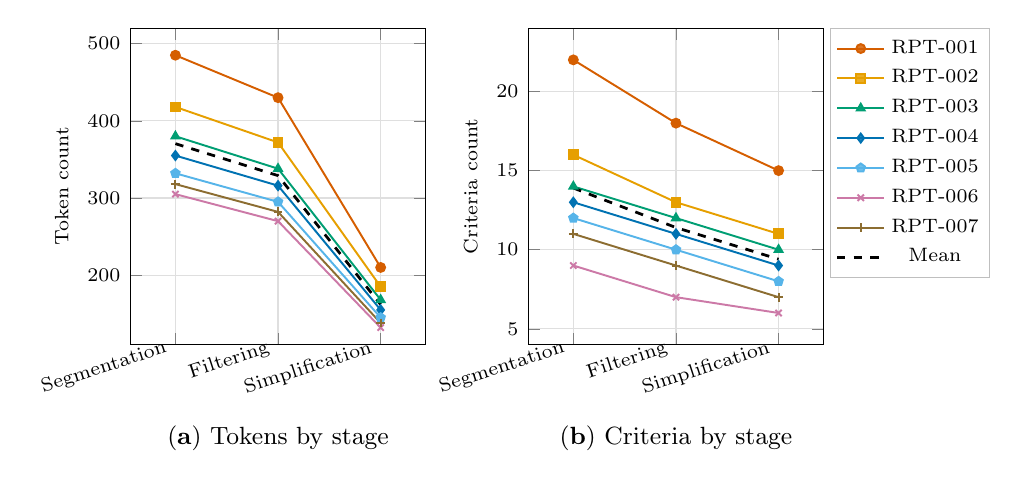
\begin{tikzpicture}
\begin{groupplot}[
  group style={group size=2 by 1, horizontal sep=13mm},
  width=0.44\linewidth, height=5.6cm,
  /tikz/font=\scriptsize,
  symbolic x coords={Segmentation,Filtering,Simplification},
  xtick=data,
  x tick label style={rotate=18,anchor=east},
  enlarge x limits=0.22,
  grid=major, grid style={gray!25},
  legend style={font=\scriptsize,draw=gray!50,fill=white,fill opacity=0.85,
                text opacity=1,at={(1.02,1.0)},anchor=north west,
                row sep=0.5pt,inner sep=2pt},
  every axis plot/.append style={mark size=1.6pt,line width=0.7pt},
  % seven distinct CVD-safe hues, one per task (default cycle reused blue/red)
  cycle list={{okVermillion},{okOrange},{okGreen},{okBlue},{okSky},{okPurple},{okGold}},
]

%------------- Panel A : tokens -------------
\nextgroupplot[ylabel={Token count},ymin=110,ymax=520,
               xlabel={\panel{a}{Tokens by stage}},
               xlabel style={yshift=-1mm}]
\addplot+[mark=*]        coordinates {(Segmentation,485)(Filtering,430)(Simplification,210)};
\addplot+[mark=square*]  coordinates {(Segmentation,418)(Filtering,372)(Simplification,185)};
\addplot+[mark=triangle*]coordinates {(Segmentation,380)(Filtering,338)(Simplification,168)};
\addplot+[mark=diamond*] coordinates {(Segmentation,355)(Filtering,316)(Simplification,155)};
\addplot+[mark=pentagon*]coordinates {(Segmentation,332)(Filtering,295)(Simplification,145)};
\addplot+[mark=x]        coordinates {(Segmentation,305)(Filtering,270)(Simplification,132)};
\addplot+[mark=+]        coordinates {(Segmentation,318)(Filtering,282)(Simplification,138)};
\addplot[black,dashed,line width=1pt,mark=none]
  coordinates {(Segmentation,370.4)(Filtering,329.0)(Simplification,161.9)};

%------------- Panel B : criteria -------------
\nextgroupplot[ylabel={Criteria count},ymin=4,ymax=24,
               xlabel={\panel{b}{Criteria by stage}},
               xlabel style={yshift=-1mm}]
\addplot+[mark=*]        coordinates {(Segmentation,22)(Filtering,18)(Simplification,15)};
\addlegendentry{RPT-001}
\addplot+[mark=square*]  coordinates {(Segmentation,16)(Filtering,13)(Simplification,11)};
\addlegendentry{RPT-002}
\addplot+[mark=triangle*]coordinates {(Segmentation,14)(Filtering,12)(Simplification,10)};
\addlegendentry{RPT-003}
\addplot+[mark=diamond*] coordinates {(Segmentation,13)(Filtering,11)(Simplification,9)};
\addlegendentry{RPT-004}
\addplot+[mark=pentagon*]coordinates {(Segmentation,12)(Filtering,10)(Simplification,8)};
\addlegendentry{RPT-005}
\addplot+[mark=x]        coordinates {(Segmentation,9)(Filtering,7)(Simplification,6)};
\addlegendentry{RPT-006}
\addplot+[mark=+]        coordinates {(Segmentation,11)(Filtering,9)(Simplification,7)};
\addlegendentry{RPT-007}
\addplot[black,dashed,line width=1pt,mark=none]
  coordinates {(Segmentation,13.9)(Filtering,11.4)(Simplification,9.4)};
\addlegendentry{Mean}
\end{groupplot}
\end{tikzpicture}
\caption{预处理各阶段中 token 数与口径条数的递减。(\textbf{a}) 七项验证任务在切分、过滤、简化三个阶段的 token 数变化。(\textbf{b}) 相应的口径条数变化。所示任务为：RPT-001（各科室月度择期手术量）、RPT-002（非计划再次手术率）、RPT-003（麻醉后监护室通过量与延迟离室率）、RPT-004（月度输血量与输血反应率）、RPT-005（检验危急值通报及时率）、RPT-006（手术部位感染监测分母）、RPT-007（日间手术占手术总量比例）。黑色虚线为各任务的均值。}
\label{fig:preproc}
\end{figure}
%%CNFLOAT-END:fig:preproc%%

这轮预处理识别出 66 条适合自动生成查询的统计口径。对这 66 条预处理后口径做信息抽取，
得到 158 个唯一业务术语，并成功映射到仓库可用的元素上。域分布分析显示，
手术麻醉类概念占比最高（n＝58，36.7\%），其后依次为登记与就诊（n＝27，17.1\%）、
诊断与病案（n＝23，14.6\%）、检验（n＝17，10.8\%）、输血（n＝13，8.2\%）、
费用与计费（n＝10，6.3\%）、人员与机构（n＝6，3.8\%）、病区与床位
（n＝4，2.5\%）（表~\ref{tab:domains}）。术语频次分析表明，时间口径类术语出现最广。
"手术入室时间"在全部 7 项任务中都出现（100.0\%；12 次提及）。
其他高频术语包括"出院日期"（6/7 项任务，85.7\%；9 次）、
"科室"（5/7，71.4\%；8 次）、"择期手术"（4/7，57.1\%；6 次）、
"非计划再次手术"（3/7，42.9\%；4 次）、"ASA 分级"（2/7，28.6\%；3 次）、
"输血反应"（2/7，28.6\%；3 次）与"并发症"（2/7，28.6\%；2 次），
见表~\ref{tab:terms}。百分比按该术语出现过的任务数计算，
"次"指该术语在任务内出现于多少条口径中。

%%CNFLOAT-BEGIN:tab:domains%%
\begin{table}[H]
\caption{抽取出的业务术语按临床数据仓库（CDW）\tnote{1}主题域的分布。}
\label{tab:domains}
\centering
\footnotesize
\begin{tabular*}{\linewidth}{@{\extracolsep{\fill}}ll@{}}
\toprule
Domains & Count (n=158), n (\%)\\
\midrule
Surgery and anesthesia        & 58 (36.7)\\
Registration and visit        & 27 (17.1)\\
Diagnosis and medical record  & 23 (14.6)\\
Laboratory                    & 17 (10.8)\\
Blood transfusion             & 13 (8.2)\\
Fee and billing               & 10 (6.3)\\
Staff and organization        & 6 (3.8)\\
Ward and bed                  & 4 (2.5)\\
\bottomrule
\end{tabular*}
\tabfoot{\tnotedef{1}CDW: clinical data warehouse.}
\end{table}
%%CNFLOAT-END:tab:domains%%

%%CNFLOAT-BEGIN:tab:terms%%
\begin{table}[H]
\caption{全部任务中出现频次最高的十个业务术语。}
\label{tab:terms}
\centering
\footnotesize
\begin{tabular*}{\linewidth}{@{\extracolsep{\fill}}lll@{}}
\toprule
Business terms & Tasks (n=7), n (\%) & Mentions (criterion), n\\
\midrule
Operation room-in time                 & 7 (100.0) & 12\\
Discharge date                         & 6 (85.7)  & 9\\
Department                             & 5 (71.4)  & 8\\
Elective surgery                       & 4 (57.1)  & 6\\
Unplanned reoperation                  & 3 (42.9)  & 4\\
ASA\tnote{1} physical status classification & 2 (28.6) & 3\\
Transfusion reaction                   & 2 (28.6)  & 3\\
Complication                           & 2 (28.6)  & 2\\
PACU\tnote{2} discharge time           & 1 (14.3)  & 2\\
Critical laboratory value              & 1 (14.3)  & 1\\
\bottomrule
\end{tabular*}
\tabfoot{\tnotedef{1}ASA: American Society of Anesthesiologists.\\
\tnotedef{2}PACU: postanesthesia care unit.}
\end{table}
%%CNFLOAT-END:tab:terms%%

\subsection{映射方法的对比表现}
在从 30 项开发任务中抽出的 398 个业务术语上，映射准确率的评估显示大模型优于 RBFM。
大模型总体准确率为 52.3\%（208/398），RBFM 为 32.9\%（131/398），
差异具有统计学意义（$P<.001$，McNemar 检验）。按域分层的分析显示，
大模型在手术麻醉域准确率最高（70.7\%，58/82），在检验域最低（34.5\%，29/84），
提示涉及数值阈值与单位解读的检验项概念尤其困难。

仅用 BM25 的参照达到 24.4\%（97/398），低于 RBFM——这在意料之中，
因为 RBFM 在字符串相似度之上还叠加了一份人工整理的同义词表；
报告它是为了让院外读者有一个自己能复现的基线。值得注意的是，
在 RBFM 分类错误的 267 个术语中，大模型正确映射了 72 个（27.0\%），
显示出更强的上下文理解。例如，RBFM 把"手术入室时间"错误映射到登记表上的
入院时间戳——一个词形接近但语义不同的字段——而大模型正确识别出麻醉记录上的
入室时间戳。这种语义解读上的改进，在多词的、承载口径的术语上是一致的。

\subsection{SQL 生成质量与专家校验}
两位领域专家用 72 条预设评价项，从 SQL 语法合规、仓库结构合规、口径上下文准确性
三个维度，独立评估了七项验证任务生成的 SQL（评分者间一致性：Cohen $\kappa$＝0.79）。
每条评价项按 4 级量表评分（1＝不合规，4＝完全合规）。SQL 语法合规获得专家高分
（3.92$\pm$0.16），大模型自评接近满分（4.00$\pm$0.00），确认了稳健的语法生成能力。
仓库结构合规同样表现良好（专家 3.78$\pm$0.28，大模型 3.98$\pm$0.06），
说明系统成功适配了分层表结构及其关联路径。

然而口径上下文准确性的波动更大、绝对分更低（专家 2.96$\pm$0.48，
大模型 3.41$\pm$0.36），0.45 分的差距提示大模型在口径解读上系统性地过度自信
（$P$＝.021，配对 $t$ 检验）。这一分歧在涉及时间选择或多条件计数逻辑的口径上最为明显。

在全部受评查询中，有 24 条含有来自开发集的预先校验口径，
可用于对映射准确性做额外验证。对这些查询，口径纳入准确性均值为
3.22$\pm$0.44（专家）对 3.45$\pm$0.33（大模型），
字段标识正确性则更高，为 3.68$\pm$0.29（专家）对 3.98$\pm$0.06（大模型）。
大模型在字段标识正确性上接近满分，反映的是它稳定生成语法有效标识的能力，
但这些标识未必就是口径上合适的那一个。

\subsection{统计结果检索表现}
用工程师认证的参考 SQL 做校验显示，表现与口径复杂度强相关（表~\ref{tab:retrieval}）。
对三项受评任务（RPT-001、RPT-002、RPT-005），我们评估了四条有参考标准可用的
统计口径。择期手术量（RPT-001）的查询检索准确率高，Jaccard 指数 0.79、
重叠系数达到 1.0，说明系统生成的结果集与参考集高度吻合。
相比之下，急诊手术量的 Jaccard 指数很低，仅 0.08，而重叠系数为 1.0——
这说明检索到的病例确实全部包含在参考集中，但参考集里有很大一部分没被覆盖；
溯源发现，模型只筛了单一的急诊标志位，而本院的定义用的是两个标志位。
非计划再次手术（RPT-002）则完全检索失败，Jaccard 指数与重叠系数均为 0，
说明没有检索到任何匹配病例。原因是系统选中了一个结构上看似合理、
但全库未填充的计划标志位，而不是手术申请表实际使用的再次手术标记——
这种失效对语法与结构校验都是不可见的。检验危急值暴露（RPT-005）表现中等，
Jaccard 指数 0.27、重叠系数 0.48，反映出对一个由数值阈值与通报记录混合表示的指标，
映射只取得了部分成功。

%%CNFLOAT-BEGIN:tab:retrieval%%
\begin{table}[H]
\caption{系统生成查询与已校验参考 SQL\tnote{1} 的结果集检索对比。}
\label{tab:retrieval}
\centering
\footnotesize
\begin{tabular*}{\linewidth}{@{\extracolsep{\fill}}llll@{}}
\toprule
Task ID & Simplified criterion & Jaccard similarity & Overlap coefficient\\
\midrule
RPT-002 & Unplanned reoperation                & 0    & 0\\
RPT-001 & Emergency surgery volume             & 0.08 & 1.0\\
        & Elective surgery volume              & 0.79 & 1.0\\
RPT-005 & Critical laboratory value exposure   & 0.27 & 0.48\\
\bottomrule
\end{tabular*}
\tabfoot{\tnotedef{1}SQL: Structured Query Language.}
\end{table}
%%CNFLOAT-END:tab:retrieval%%

在这四条口径上，系统在唯一那条定义明确的单口径指标（择期手术量）上表现良好，
而在另外三条上表现不佳——它们的定义或是复合的、或是院内特有的、
或依赖一个填充稀疏的字段（急诊手术量、非计划再次手术、检验危急值暴露）。
来自三项任务的四条口径不足以确立这一反差可以推广；
我们把它作为一次个案系列报告，用以引出错误分析，而不是作为"系统在哪里成功"的估计。
要提升更复杂统计口径的检索表现，可能需要改进口径字典的覆盖面与字段填充情况的画像。

\subsection{大规模模型对比与幻觉分析}
为系统评估多个大模型的幻觉模式，我们在 SynHDW 上另做了一次大规模实验，
分析 960 次 SQL 生成尝试（24 项报表任务 $\times$ 8 个模型 $\times$ 5 种提示策略），
与前面的初始验证研究相互独立。对这 960 次尝试的分析显示模型间表现差异显著
（$F_{7,783}$＝4.18，$P<.001$）。这项总体检验有一点需要说明：
phi3 只在 18.3\% 的尝试中产出了 SQL，把一个如此退化的组纳入进来会抬高组间方差。
在 SQL 生成成功率 $>$80\% 的模型中，幻觉率介于 20.4\%（n＝22/108）与
47.1\%（n＝49/104）之间。总体幻觉率为 34.6\%（n＝274/791 条生成查询）
（95\% CI 31.4\%--38.0\%）。由于这一合并把生成率相差五倍的模型放在一起，
我们另报告限定于生成率超过 80\% 的那七个模型的结果：
35.4\%（n＝272/769；95\% CI 32.1\%--38.8\%）。两个估计相差 0.7 个百分点，
因此合并值并非纳入退化模型所导致的假象。各模型在生成能力与准确性两方面
差异都很大（图~\ref{fig:models} 与表~\ref{tab:modelperf}）。

%%CNFLOAT-BEGIN:fig:models%%
\begin{figure}[H]
\begin{adjustwidth}{-\extralength}{0cm}
\centering
\vspace{2pt}

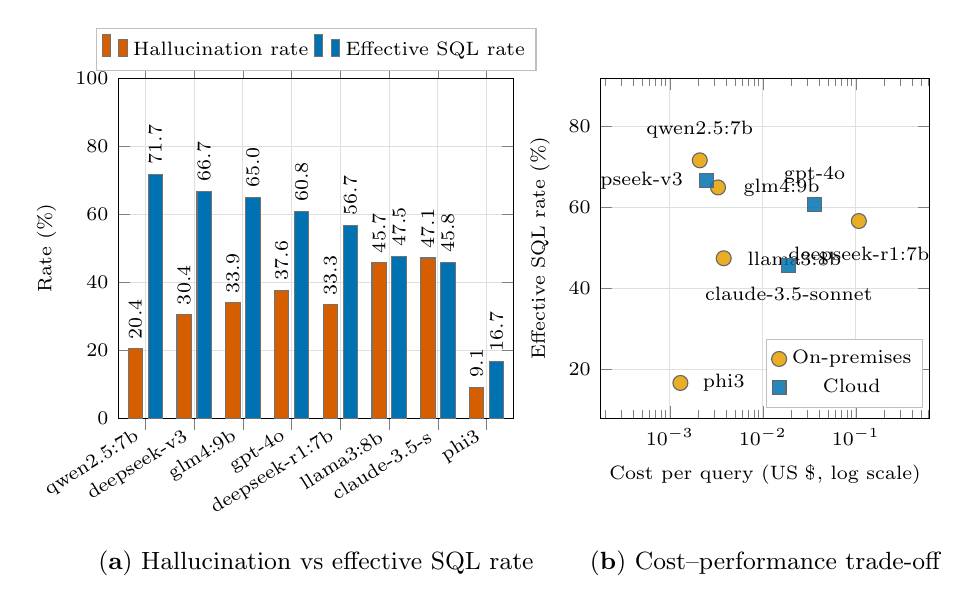
\begin{tikzpicture}
%------------- Panel A -------------
\begin{scope}[local bounding box=bbA]
\begin{axis}[
  name=panelA,
  width=0.545\linewidth, height=5.9cm, font=\scriptsize,
  ybar, bar width=5.2pt,
  symbolic x coords={qwen2.5:7b,deepseek-v3,glm4:9b,gpt-4o,deepseek-r1:7b,
                     llama3:8b,claude-3.5-s,phi3},
  xtick=data, x tick label style={rotate=32,anchor=east,font=\scriptsize},
  ymin=0, ymax=100, ylabel={Rate (\%)},
  grid=major, grid style={gray!25},
  legend style={font=\scriptsize,at={(0.5,1.02)},anchor=south,legend columns=2,
                draw=gray!50,inner sep=2pt},
  enlarge x limits=0.08,
  nodes near coords={\pgfmathprintnumber[fixed,fixed zerofill,precision=1]{\pgfplotspointmeta}},
  every node near coord/.append style={font=\scriptsize,rotate=90,anchor=west},
]
\addplot[fill=okVermillion,draw=black!55] coordinates {
  (qwen2.5:7b,20.4) (deepseek-v3,30.4) (glm4:9b,33.9) (gpt-4o,37.6)
  (deepseek-r1:7b,33.3) (llama3:8b,45.7) (claude-3.5-s,47.1) (phi3,9.1)};
\addlegendentry{Hallucination rate}
\addplot[fill=okBlue,draw=black!55] coordinates {
  (qwen2.5:7b,71.7) (deepseek-v3,66.7) (glm4:9b,65.0) (gpt-4o,60.8)
  (deepseek-r1:7b,56.7) (llama3:8b,47.5) (claude-3.5-s,45.8) (phi3,16.7)};
\addlegendentry{Effective SQL rate}
\end{axis}
\end{scope}

%------------- Panel B -------------
\begin{scope}[local bounding box=bbB]
\begin{axis}[
  name=panelB, at={($(panelA.east)+(11mm,0)$)}, anchor=west,
  width=0.475\linewidth, height=5.9cm, font=\scriptsize,
  xmode=log, log basis x=10,
  xlabel={Cost per query (US \$, log scale)},
  ylabel={Effective SQL rate (\%)},
  xmin=0.00018, xmax=0.62, ymin=8, ymax=92,
  grid=major, grid style={gray!25},
  legend style={font=\scriptsize,at={(0.98,0.03)},anchor=south east,draw=gray!50,inner sep=2pt},
]
% on-premises models (orange)
\addplot[only marks, mark=*, mark size=2.7pt,
         mark options={draw=black!60,fill=okOrange,fill opacity=0.85}]
  table[x=x,y=y] {
x        y     sz
0.0021   71.7  6.5
0.0033   65.0  6.0
0.1078   56.7  5.3
0.0038   47.5  4.6
0.0013   16.7  2.1
};
\addlegendentry{On-premises}
% cloud models (blue)
\addplot[only marks, mark=square*, mark size=2.5pt,
         mark options={draw=black!60,fill=okBlue,fill opacity=0.85}]
  table[x=x,y=y] {
x        y     sz
0.0025   66.7  6.1
0.0190   45.8  4.5
0.0360   60.8  5.7
};
\addlegendentry{Cloud}
% annotations (placed to avoid mutual overlap and axis-edge clipping)
\node[font=\scriptsize,anchor=south,yshift=1.6mm]      at (axis cs:0.0021,71.7) {qwen2.5:7b};
\node[font=\scriptsize,anchor=east,xshift=-1.8mm]      at (axis cs:0.0025,66.7) {deepseek-v3};
\node[font=\scriptsize,anchor=south,yshift=1.4mm]      at (axis cs:0.0360,60.8) {gpt-4o};
\node[font=\scriptsize,anchor=west,xshift=2.0mm]       at (axis cs:0.0033,65.0) {glm4:9b};
\node[font=\scriptsize,anchor=north,yshift=-2.0mm]     at (axis cs:0.1078,56.7) {deepseek-r1:7b};
\node[font=\scriptsize,anchor=west,xshift=1.8mm]       at (axis cs:0.0038,47.5) {llama3:8b};
\node[font=\scriptsize,anchor=north,yshift=-1.6mm]     at (axis cs:0.0190,45.8) {claude-3.5-sonnet};
\node[font=\scriptsize,anchor=west,xshift=1.6mm]       at (axis cs:0.0013,16.7) {phi3};
\end{axis}
\end{scope}
% MDPI panel labels: centred under each panel, on one common baseline
\coordinate (lbly) at ([yshift=-1.4mm]current bounding box.south);
\node[anchor=north] at (panelA.center |- lbly) {\panel{a}{Hallucination vs effective SQL rate}};
\node[anchor=north] at (panelB.center |- lbly) {\panel{b}{Cost--performance trade-off}};
\end{tikzpicture}
\caption{八个大语言模型在临床数据仓库（CDW）结构化查询语言（SQL）生成上的表现。(\textbf{a}) 各模型的幻觉率与有效 SQL 率，每个模型 120 次尝试。(\textbf{b}) 每次查询成本对有效 SQL 率；云端模型画为蓝色方块，本地模型画为橙色圆点。本地模型没有按次 API 费用，图中按摊薄成本作图，即推理时间 $\times$ 每 GPU 小时 0.28 美元（按本院 3 年硬件摊销计）。}
\label{fig:models}
\end{adjustwidth}
\end{figure}
%%CNFLOAT-END:fig:models%%

%%CNFLOAT-BEGIN:tab:modelperf%%
\begin{table}[H]
\begin{adjustwidth}{-\extralength}{0cm}
\caption{模型表现汇总。}
\label{tab:modelperf}
\centering
\footnotesize
\setlength{\tabcolsep}{4pt}
\begin{tabular*}{\linewidth}{@{\extracolsep{\fill}}L{3.3cm}L{2.0cm}L{2.0cm}L{2.1cm}L{2.0cm}L{2.5cm}L{2.0cm}@{}}
\toprule
Model & Architec\-ture & SQL\tnote{1} genera\-tion (\%) & Halluci\-nation (\%)\tnote{2}
      & Effec\-tive SQL (\%)\tnote{3} & Time (s)\tnote{4} & Cost (US \$)/Query\\
\midrule
qwen2.5:7b        & On-premises & 90.0  & 20.4          & 71.7 & 27.3$\pm$6.4      & 0.000\\
deepseek-v3       & Cloud       & 95.8  & 30.4          & 66.7 & 7.6$\pm$1.9       & 0.003\\
glm4:9b           & On-premises & 98.3  & 33.9          & 65.0 & 41.8$\pm$10.2     & 0.000\\
gpt-4o            & Cloud       & 97.5  & 37.6          & 60.8 & 18.5$\pm$4.3      & 0.036\\
deepseek-r1:7b    & On-premises & 85.0  & 33.3          & 56.7 & 1386.2$\pm$352.4  & 0.000\\
llama3:8b         & On-premises & 87.5  & 45.7          & 47.5 & 48.7$\pm$12.1     & 0.000\\
claude-3.5-sonnet & Cloud       & 86.7  & 47.1          & 45.8 & 14.1$\pm$3.6      & 0.019\\
phi3              & On-premises & 18.3  & 9.1\tnote{5}  & 16.7 & 16.9$\pm$6.8      & 0.000\\
\bottomrule
\end{tabular*}
\tabfoot{\tnotedef{1}SQL: Structured Query Language.\\
\tnotedef{2}Percentage of generated queries with invalid field identifiers or
criterion assignments.\\
\tnotedef{3}SQL generation $\times$ (1--hallucination).\\
\tnotedef{4}Mean$\pm$SD.\\
\tnotedef{5}Misleading due to low generation rate.}
\end{adjustwidth}
\end{table}
%%CNFLOAT-END:tab:modelperf%%

qwen2.5:7b 成为最有效的模型，有效 SQL 率 71.7\%（95\% CI 63.0\%--79.0\%），
尽管其 SQL 生成能力只属中等（90.0\%）；原因是它幻觉率低（20.4\%）
且极少使用占位符（22.7\%）。相比之下，gpt-4o 生成率很高（97.5\%），
有效率却较低（60.8\%，95\% CI 51.9\%--69.1\%），因为它大量使用占位符（31.8\%），
并且在所需统计口径未被明示时，明显倾向于代入一个看似合理的时间戳。

\subsection{幻觉模式分析}
对 274 条幻觉的分类显示各模型有不同的错误模式（图~\ref{fig:halluc}）。
Category B（错误的口径指派）占比最高（34.7\%，n＝95），
其次为 Category D（占位符插入，28.5\%，n＝78）与
Category E（结构与方言错误，24.5\%，n＝67）。
Category A（不存在的字段标识）相对少见（9.9\%，n＝27），
Category C（自然语言替代）亦然（2.6\%，n＝7）。$\chi^2$ 分析确认各模型的错误分布
差异显著（$\chi^2$＝48.2，$df$＝28，$P$＝.009）。

%%CNFLOAT-BEGIN:fig:halluc%%
\begin{figure}[H]
\begin{adjustwidth}{-\extralength}{0cm}
\centering
\vspace{2pt}

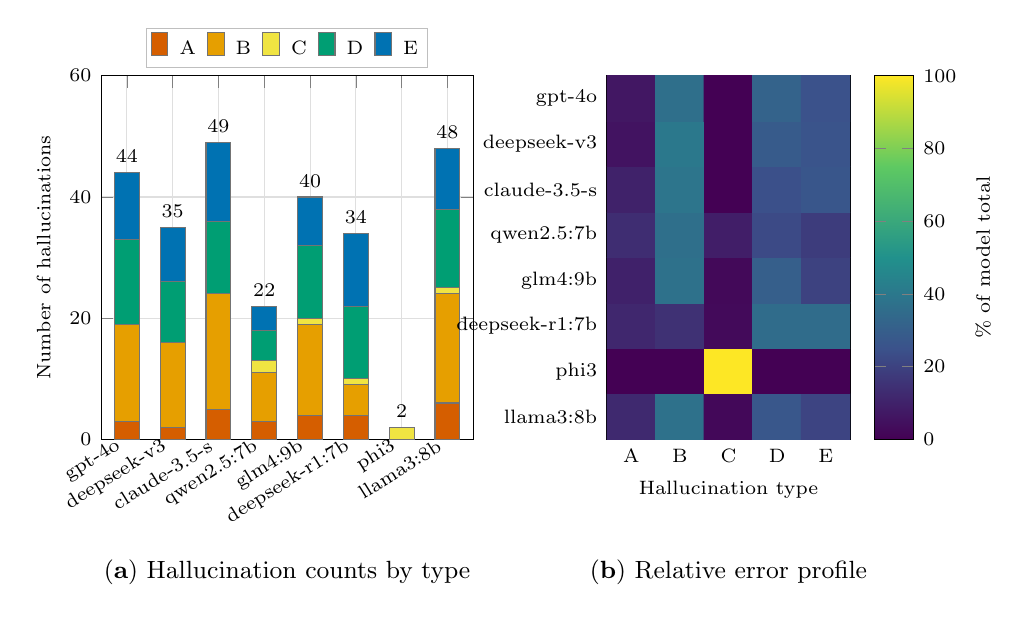
\begin{tikzpicture}
%------------- Panel A : stacked bars -------------
\begin{scope}[local bounding box=bbA]
\begin{axis}[
  name=hA,
  width=0.52\linewidth, height=6.2cm, font=\scriptsize,
  ybar stacked, bar width=9pt,
  symbolic x coords={gpt-4o,deepseek-v3,claude-3.5-s,qwen2.5:7b,glm4:9b,
                     deepseek-r1:7b,phi3,llama3:8b},
  xtick=data, x tick label style={rotate=32,anchor=east,font=\scriptsize},
  ymin=0, ymax=60, ylabel={Number of hallucinations},
  grid=major, grid style={gray!25},
  legend style={font=\scriptsize,at={(0.5,1.02)},anchor=south,legend columns=5,
                draw=gray!50,inner sep=1.5pt,column sep=2pt},
  enlarge x limits=0.08,
]
\addplot[fill=okVermillion,draw=black!55]     coordinates {(gpt-4o,3)(deepseek-v3,2)(claude-3.5-s,5)(qwen2.5:7b,3)(glm4:9b,4)(deepseek-r1:7b,4)(phi3,0)(llama3:8b,6)};
\addlegendentry{A}
\addplot[fill=okOrange,draw=black!55]  coordinates {(gpt-4o,16)(deepseek-v3,14)(claude-3.5-s,19)(qwen2.5:7b,8)(glm4:9b,15)(deepseek-r1:7b,5)(phi3,0)(llama3:8b,18)};
\addlegendentry{B}
\addplot[fill=okYellow,draw=black!55]  coordinates {(gpt-4o,0)(deepseek-v3,0)(claude-3.5-s,0)(qwen2.5:7b,2)(glm4:9b,1)(deepseek-r1:7b,1)(phi3,2)(llama3:8b,1)};
\addlegendentry{C}
\addplot[fill=okGreen,draw=black!55]    coordinates {(gpt-4o,14)(deepseek-v3,10)(claude-3.5-s,12)(qwen2.5:7b,5)(glm4:9b,12)(deepseek-r1:7b,12)(phi3,0)(llama3:8b,13)};
\addlegendentry{D}
\addplot[fill=okBlue,draw=black!55]    coordinates {(gpt-4o,11)(deepseek-v3,9)(claude-3.5-s,13)(qwen2.5:7b,4)(glm4:9b,8)(deepseek-r1:7b,12)(phi3,0)(llama3:8b,10)};
\addlegendentry{E}
% totals above bars
\node[font=\scriptsize,anchor=south] at (axis cs:gpt-4o,44) {44};
\node[font=\scriptsize,anchor=south] at (axis cs:deepseek-v3,35) {35};
\node[font=\scriptsize,anchor=south] at (axis cs:claude-3.5-s,49) {49};
\node[font=\scriptsize,anchor=south] at (axis cs:qwen2.5:7b,22) {22};
\node[font=\scriptsize,anchor=south] at (axis cs:glm4:9b,40) {40};
\node[font=\scriptsize,anchor=south] at (axis cs:deepseek-r1:7b,34) {34};
\node[font=\scriptsize,anchor=south] at (axis cs:phi3,2) {2};
\node[font=\scriptsize,anchor=south] at (axis cs:llama3:8b,48) {48};
\end{axis}
\end{scope}

%------------- Panel B : heatmap -------------
\begin{scope}[local bounding box=bbB]
\begin{axis}[
  name=hB, at={($(hA.east)+(17mm,0)$)}, anchor=west,
  width=0.385\linewidth, height=6.2cm, font=\scriptsize,
  colormap={vlike}{rgb255=(68,1,84) rgb255=(59,82,139) rgb255=(33,145,140)
                   rgb255=(94,201,98) rgb255=(253,231,37)},
  colorbar,
  colorbar style={font=\scriptsize,ylabel={\% of model total},ylabel style={font=\scriptsize}},
  point meta min=0, point meta max=100,
  xtick={0,1,2,3,4}, xticklabels={A,B,C,D,E},
  ytick={0,1,2,3,4,5,6,7},
  yticklabels={llama3:8b,phi3,deepseek-r1:7b,glm4:9b,qwen2.5:7b,
               claude-3.5-s,deepseek-v3,gpt-4o},
  y tick label style={font=\scriptsize},
  xlabel={Hallucination type},
  enlarge x limits=false, enlarge y limits=false,
]
\addplot[matrix plot*, point meta=explicit, mesh/cols=5] table[meta=v] {
x y v
0 0 12.5
1 0 37.5
2 0 2.1
3 0 27.1
4 0 20.8
0 1 0.0
1 1 0.0
2 1 100.0
3 1 0.0
4 1 0.0
0 2 11.8
1 2 14.7
2 2 2.9
3 2 35.3
4 2 35.3
0 3 10.0
1 3 37.5
2 3 2.5
3 3 30.0
4 3 20.0
0 4 13.6
1 4 36.4
2 4 9.1
3 4 22.7
4 4 18.2
0 5 10.2
1 5 38.8
2 5 0.0
3 5 24.5
4 5 26.5
0 6 5.7
1 6 40.0
2 6 0.0
3 6 28.6
4 6 25.7
0 7 6.8
1 7 36.4
2 7 0.0
3 7 31.8
4 7 25.0
};
\end{axis}
\end{scope}
% MDPI panel labels: centred under each panel, on one common baseline
\coordinate (lbly) at ([yshift=-1.4mm]current bounding box.south);
\node[anchor=north] at (hA.center |- lbly) {\panel{a}{Hallucination counts by type}};
\node[anchor=north] at (hB.center |- lbly) {\panel{b}{Relative error profile}};
\end{tikzpicture}
\caption{各模型的幻觉类型分布，基于 274 条含幻觉的查询。(\textbf{a}) 各模型每类幻觉的绝对计数，堆叠显示，柱上方为该模型合计。类型为 A，不存在的字段标识；B，错误的口径指派；C，标识位置上的自然语言；D，占位符插入；E，结构与方言错误。(\textbf{b}) 同一批计数按各模型自身合计的百分比显示，以便在不受错误总量影响的情况下比较错误构成；颜色越深表示占该模型合计的比例越小。两个面板中模型顺序相同。}
\label{fig:halluc}
\end{adjustwidth}
\end{figure}
%%CNFLOAT-END:fig:halluc%%

按模型细看可见各自特有的失效方式（表~\ref{tab:halluctypes}）。
claude-3.5-sonnet 的基线幻觉率最高（47.1\%），但在 error\_aware 提示下改善显著
（幻觉率 18.5\%，相对下降 60.7\%）。deepseek-v3 在 explicit\_uncertainty 提示下
达到 96.0\% 的有效 SQL 率，不过仅限于简单的单表计数查询。
phi3 表面上很低的幻觉率（9.1\%）具有误导性——它来自 81.7\% 的"根本没产出 SQL"，
而不是来自准确生成。

%%CNFLOAT-BEGIN:tab:halluctypes%%
\begin{table}[H]
\begin{adjustwidth}{-\extralength}{0cm}
\caption{各模型幻觉类型的详细分布。}
\label{tab:halluctypes}
\centering
\footnotesize
\setlength{\tabcolsep}{4pt}
\begin{tabular*}{\linewidth}{@{\extracolsep{\fill}}L{3.1cm}L{2.05cm}L{2.2cm}L{2.2cm}L{2.2cm}L{2.05cm}L{2.05cm}@{}}
\toprule
Model & Total halluci\-nations & Category A (nonexis\-tent), n (\%)
      & Category B (wrong criterion), n (\%)
      & Category C (natural language), n (\%)
      & Category D (place\-holder), n (\%)
      & Category E (schema errors), n (\%)\\
\midrule
gpt-4o            & 44 & 3 (6.8)  & 16 (36.4) & 0 (0)     & 14 (31.8) & 11 (25.0)\\
deepseek-v3       & 35 & 2 (5.7)  & 14 (40.0) & 0 (0)     & 10 (28.6) & 9 (25.7)\\
claude-3.5-sonnet & 49 & 5 (10.2) & 19 (38.8) & 0 (0)     & 12 (24.5) & 13 (26.5)\\
qwen2.5:7b        & 22 & 3 (13.6) & 8 (36.4)  & 2 (9.1)   & 5 (22.7)  & 4 (18.2)\\
glm4:9b           & 40 & 4 (10.0) & 15 (37.5) & 1 (2.5)   & 12 (30.0) & 8 (20.0)\\
deepseek-r1:7b    & 34 & 4 (11.8) & 5 (14.7)  & 1 (2.9)   & 12 (35.3) & 12 (35.3)\\
phi3              & 2  & 0 (0)    & 0 (0)     & 2 (100)   & 0 (0)     & 0 (0)\\
llama3:8b         & 48 & 6 (12.5) & 18 (37.5) & 1 (2.1)   & 13 (27.1) & 10 (20.8)\\
\bottomrule
\end{tabular*}
\end{adjustwidth}
\end{table}
%%CNFLOAT-END:tab:halluctypes%%

Tukey HSD 事后分析显示模型之间的有效 SQL 生成率存在显著的两两差异。
qwen2.5:7b 显著优于 gpt-4o（均值差 10.8 个百分点，$P$＝.021），
效应量为中到大（Cohen $d$＝0.74）。最好（qwen2.5:7b）与最差（phi3）之间的差距很大
（$d$＝2.71），说明差异在统计显著之外还具有实际意义。

\subsection{提示工程的影响}
对提示策略的评估显示，相对 zero\_shot 基线，所有其他策略都产生了较大的效应量
（Cohen $d>$1.0）。尽管效应量大，模型与提示交互的高方差使得主效应未能被检出
（$F_{4,955}$＝1.58，$P$＝.178）。明确点出 SynHDW 覆盖限制与常见陷阱的
error\_aware 策略，对高幻觉模型最为有效；而 explicit\_uncertainty 则在
需要保守解读的较简单查询上表现突出。

\subsection{提示策略表现分析}
对全部 8 个模型的提示策略做综合分析（每种提示 192 条查询），
在幻觉控制上呈现出意料之外的模式。由于提示策略的总体检验不显著，
下面的排序是描述性的、两两对比是探索性的；二者都不作为"某一策略优于另一策略"的
确证证据。zero\_shot 表现最好，幻觉率最低（均值 17.4\%，SD 13.2\%）、
有效 SQL 率最高（均值 67.1\%，SD 19.8\%），显著优于更复杂的策略。
相反，提供了详细逐步子结构指引的 structured\_approach 幻觉率最高
（均值 39.6\%，SD 22.4\%）、有效率最低（均值 46.8\%，SD 18.1\%）。
本为强调准确性而设计的 validation\_focused 反而使表现低于 zero\_shot
（$P$＝.046，Tukey HSD），有效 SQL 率均值（SD）仅为 53.7\%（20.9\%）。
其余两种居中：error\_aware 的幻觉率均值（SD）为 23.1\%（14.8\%）、
有效率 60.4\%（17.7\%）；explicit\_uncertainty 分别为 26.8\%（17.5\%）与
59.2\%（20.6\%）。这些结果提示，在分层仓库结构上做基于大模型的 SQL 生成时，
过多的指令复杂度带来的可能是混淆而非清晰。

各项指标上都很大的标准差（13.2\% 至 22.4\%）说明模型对提示的响应存在显著的
个体差异。例如同样用 zero\_shot 提示，deepseek-r1:7b 的幻觉率为 2.1\%，
而 claude-3.5-sonnet 为 41.5\%，相差 39.4 个百分点。
回归分析进一步确认了这一点：模型身份解释了 61\% 的表现方差
（$R^2$＝0.61，$P<.001$），而提示策略的贡献很小。
需要说明的是，这里的"模型身份"混杂了部署方式、参数量、模型家族、
以及是否为推理导向等因素；本设计无法把它们分开，
因此该方差应归于"整体的模型选择"，而不是具体归因于架构。
据此可以指出较优的模型--提示组合：qwen2.5:7b 配 zero\_shot 达到 79.2\% 的有效 SQL 率；
deepseek-v3 配 explicit\_uncertainty 在简单的单表计数查询上达到 96.0\% 的有效率，
但对口径敏感的指标适用性有限。

\subsection{弃权质量}\label{sec:cn-abst}
在 791 条生成查询中，系统共 132 次提出 TO-CONFIRM 条目，触发率 16.7\%。
其中 104 次是应当提出的，弃权精确率为 78.8\%；其余 28 次询问的是工程师判定为
并无歧义的口径。另有 61 条真有歧义的口径被系统自行决定，
因此系统在 165 条有歧义的情形中识别出 104 条，召回率 63.0\%。
漏弃权是这个数字里更要紧的那一半：在这 61 条中有 42 条，系统所采纳的读法
并不是工程师会选的那一种；这占表~\ref{tab:halluctypes} 中 95 条错误口径的 44.2\%。
其余 53 条错误口径出现在口径本无歧义、系统只是映射错了的情形。

弃权行为与幻觉控制同向变化，而不是独立变动（表~\ref{tab:abstain}）。
幻觉率最低的 qwen2.5:7b，既弃权最频繁（占其生成查询的 22.2\%）、
也弃权最准（87.5\%），且只漏掉 5 条有歧义口径。
在生成率超过 80\% 的模型中幻觉率最高的 llama3:8b，弃权最少（13.3\%）、
最不准（71.4\%），漏掉 11 条。一个不善于识别"字段映射错了"的模型，
看来同样不善于识别"这条口径无法判定"。

%%CNFLOAT-BEGIN:tab:abstain%%
\begin{table}[H]
\caption{各模型的弃权行为。触发率为 TO-CONFIRM 条目占该模型生成查询数的比例；精确率为应当弃权者占所提出弃权的比例；漏弃权指模型未加询问即自行决定的有歧义口径。}
\label{tab:abstain}
\centering
\footnotesize
\setlength{\tabcolsep}{5pt}
\begin{tabular*}{\linewidth}{@{\extracolsep{\fill}}llllll@{}}
\toprule
Model & Generated, n & Triggered, n (\%) & Warranted, n (\%) & Missed, n & Recall, \%\\
\midrule
qwen2.5:7b        & 108 & 24 (22.2) & 21 (87.5) & 5  & 80.8\\
deepseek-v3       & 115 & 19 (16.5) & 15 (78.9) & 8  & 65.2\\
gpt-4o            & 117 & 21 (17.9) & 16 (76.2) & 8  & 66.7\\
glm4:9b           & 118 & 18 (15.3) & 14 (77.8) & 9  & 60.9\\
deepseek-r1:7b    & 102 & 17 (16.7) & 13 (76.5) & 7  & 65.0\\
claude-3.5-sonnet & 104 & 17 (16.3) & 13 (76.5) & 12 & 52.0\\
llama3:8b         & 105 & 14 (13.3) & 10 (71.4) & 11 & 47.6\\
phi3              & 22  & 2 (9.1)   & 2 (100.0) & 1  & 66.7\\
\midrule
Total             & 791 & 132 (16.7) & 104 (78.8) & 61 & 63.0\\
\bottomrule
\end{tabular*}
\end{table}
%%CNFLOAT-END:tab:abstain%%

\subsection{组件消融}
每一层都有贡献，而且贡献并不重叠（表~\ref{tab:ablation}、图~\ref{fig:ablation}）。
裸模型的有效 SQL 率为 22.5\%。加入仓库结构后升到 40.8\%，
再加元数据知识库上的检索升到 60.8\%，再加四层校验升到 71.7\%。

按错误类别拆开，可以看出每一层各自消掉了什么。不存在的字段标识从设置 A 的 21 条，
在提供结构后降到 6 条，此后为 3 条：注入结构基本消除了通用 text-to-SQL 工作
所优化的那一类错误。错误的统计口径则表现不同：加入结构后它反而从 12 条升到 22 条——
因为一个现在知道真实列名的模型，会把标识错误换成口径错误——
只有检索把它折半，降到 11 条。占位符插入与方言错误合计从 7 条增至 15 条，
因为更早的失效被消除后，残余错误转移到了更轻的类别上；
随后在执行反馈下降到 9 条。因此，对本问题特有的那类错误起作用的是\emph{检索}，
不是校验；校验的作用是把剩下的机械性毛病转化为可交付的查询。

%%CNFLOAT-BEGIN:tab:ablation%%
\begin{table}[H]
\caption{qwen2.5:7b 上的组件消融。每个设置都在同样的 24 项任务与 5 种提示策略下运行，每设置 120 次尝试。设置 D 即主实验中的 qwen2.5:7b 条件。错误类别为 A，不存在的字段标识；B，错误的统计口径；C，标识位置上的自然语言；D，占位符插入；E，结构与方言错误。}
\label{tab:ablation}
\centering
\footnotesize
\setlength{\tabcolsep}{4pt}
\begin{tabular*}{\linewidth}{@{\extracolsep{\fill}}lllllllllll@{}}
\toprule
Setting & Generated & Halluc. & Gen., \% & Halluc., \% & Effective, \% & A & B & C & D & E\\
\midrule
A: bare model            & 71  & 44 & 59.2 & 62.0 & 22.5 & 21 & 12 & 4 & 5 & 2\\
B: + schema              & 92  & 43 & 76.7 & 46.7 & 40.8 & 6  & 22 & 3 & 8 & 4\\
C: + retrieval           & 104 & 31 & 86.7 & 29.8 & 60.8 & 3  & 11 & 2 & 9 & 6\\
D: + verification (full) & 108 & 22 & 90.0 & 20.4 & 71.7 & 3  & 8  & 2 & 5 & 4\\
\bottomrule
\end{tabular*}
\end{table}
%%CNFLOAT-END:tab:ablation%%

%%CNFLOAT-BEGIN:fig:ablation%%
\begin{figure}[H]
\begin{adjustwidth}{-\extralength}{0cm}
\centering

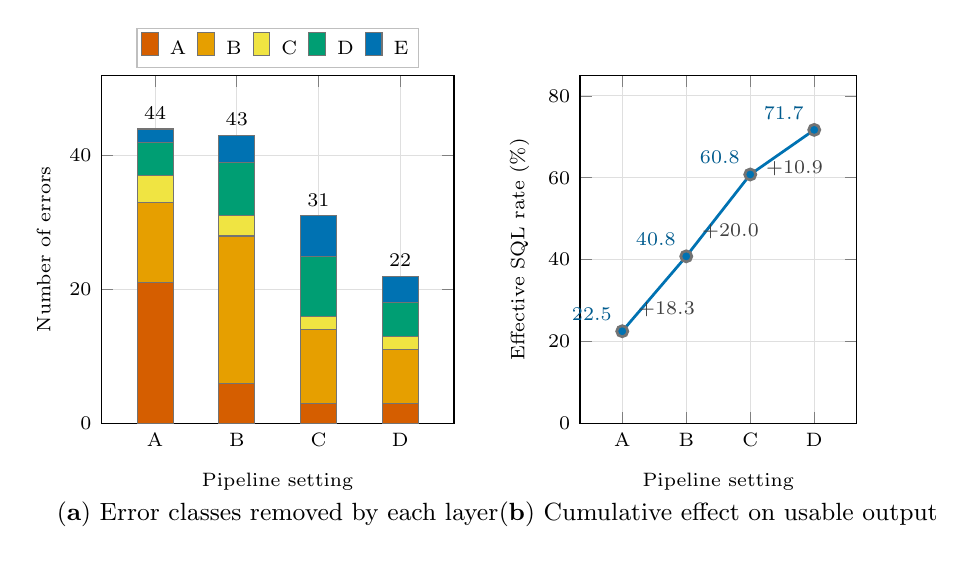
\begin{tikzpicture}
%------------- Panel A : error classes across settings -------------
\begin{axis}[
  name=abA,
  width=0.50\linewidth, height=6.0cm, font=\scriptsize,
  ybar stacked, bar width=13pt,
  symbolic x coords={A,B,C,D}, xtick=data,
  xlabel={Pipeline setting\\[3pt]\panel{a}{Error classes removed by each layer}},
  xlabel style={align=center,yshift=-1mm}, ylabel={Number of errors},
  ymin=0, ymax=52, grid=major, grid style={gray!25},
  legend style={font=\scriptsize,at={(0.5,1.02)},anchor=south,legend columns=5,
                draw=gray!50,inner sep=1.5pt,column sep=2pt},
  enlarge x limits=0.22,
]
\addplot[fill=okVermillion,draw=black!55] coordinates {(A,21)(B,6)(C,3)(D,3)};  \addlegendentry{A}
\addplot[fill=okOrange,draw=black!55]     coordinates {(A,12)(B,22)(C,11)(D,8)}; \addlegendentry{B}
\addplot[fill=okYellow,draw=black!55]     coordinates {(A,4)(B,3)(C,2)(D,2)};   \addlegendentry{C}
\addplot[fill=okGreen,draw=black!55]      coordinates {(A,5)(B,8)(C,9)(D,5)};   \addlegendentry{D}
\addplot[fill=okBlue,draw=black!55]       coordinates {(A,2)(B,4)(C,6)(D,4)};   \addlegendentry{E}
\node[font=\scriptsize,anchor=south] at (axis cs:A,44) {44};
\node[font=\scriptsize,anchor=south] at (axis cs:B,43) {43};
\node[font=\scriptsize,anchor=south] at (axis cs:C,31) {31};
\node[font=\scriptsize,anchor=south] at (axis cs:D,22) {22};
\end{axis}

%------------- Panel B : effective SQL rate -------------
\begin{axis}[
  name=abB, at={($(abA.east)+(16mm,0)$)}, anchor=west,
  width=0.42\linewidth, height=6.0cm, font=\scriptsize,
  symbolic x coords={A,B,C,D}, xtick=data,
  xlabel={Pipeline setting\\[3pt]\panel{b}{Cumulative effect on usable output}},
  xlabel style={align=center,yshift=-1mm}, ylabel={Effective SQL rate (\%)},
  ymin=0, ymax=85, grid=major, grid style={gray!25},
  enlarge x limits=0.22,
  nodes near coords={\pgfmathprintnumber[fixed,fixed zerofill,precision=1]{\pgfplotspointmeta}},
  every node near coord/.append style={font=\scriptsize,anchor=south east,text=okBlue!80!black},
]
\addplot[okBlue,mark=*,mark options={fill=okBlue,draw=black!55},line width=1pt]
  coordinates {(A,22.5)(B,40.8)(C,60.8)(D,71.7)};
% increments drawn on the segment midpoints, offset clear of the line
\node[font=\scriptsize,anchor=north west,text=black!75]
  at (axis cs:A,32.0) {\;$+18.3$};
\node[font=\scriptsize,anchor=north west,text=black!75]
  at (axis cs:B,51.0) {\;$+20.0$};
\node[font=\scriptsize,anchor=north west,text=black!75]
  at (axis cs:C,66.5) {\;$+10.9$};
\end{axis}
\end{tikzpicture}

\caption{qwen2.5:7b 上的组件消融。设置 A 为裸模型，B 加上仓库结构，C 加上在元数据知识库上的检索，D 加上四层执行反馈校验。(\textbf{a}) 按类别的绝对错误计数，柱上方为合计；错误类别为 A，不存在的字段标识；B，错误的统计口径；C，标识位置上的自然语言；D，占位符插入；E，结构与方言错误。注入仓库结构消除了 A 类错误，却使 B 类错误增加，而只有检索能把 B 类降下来。(\textbf{b}) 有效 SQL 率，并标出每一层各自贡献的增量。}
\label{fig:ablation}
\end{adjustwidth}
\end{figure}
%%CNFLOAT-END:fig:ablation%%

\subsection{公开基准参照}\label{sec:cn-bench}
在 EHRSQL 2024 开发集上，未作修改的流水线（用 qwen2.5:7b）取得 58.4\% 的执行准确率，
幻觉率 12.6\%。这个幻觉率大约是我们仓库上所观察到的一半，
这与结构规模和口径歧义程度的差异是一致的：公开结构暴露的列少得多，
而且它的问题在单一读法下就可以回答。报告这个数字是为了把本流水线的绝对水平
放到该数据集上已发表工作的参照系里；这不是在一个系统本非为其设计的基准上
主张竞争力。

\subsection{合成数据校验}
为评估所生成 SQL 的实用可行性，我们把生成成功的查询在含 112\,680 条患者记录的
SynHDW 合成数据集上执行。系统在两项已校验的报表任务上共匹配到 8250 名合成患者：
RPT-001（月度择期手术量）匹配 2840 名（占数据集 2.5\%），
RPT-004（月度输血量）匹配 5410 名（占 4.8\%）。这些结果集规模与生产报表中
观察到的月度体量相符，说明了技术可行性；不过我们也承认，
由于合成数据没有真实医院系统固有的数据质量问题——缺失值、被回溯修正的时间戳、
以及跨院区的编码差异——合成校验可能高估真实世界的表现。

%==============================================================================
\section{讨论}
%==============================================================================
\subsection{主要发现}
我们开发了一套完整框架，把自由文本的医院统计需求自动转成三层 CDW 上的
Presto SQL。系统最初是用 gpt-4o 开发的，但覆盖 8 个大模型的系统评测给出了
意料之外的结果：本地部署的 qwen2.5:7b 取得了最高的有效 SQL 生成率（71.7\%），
高于 gpt-4o 的 60.8\%，主要原因是幻觉率更低（20.4\% 对 37.6\%）。
也就是说，一个更小的、本地托管的模型胜过了一个最先进的商业模型。
把它们分开的是幻觉控制，不是原始生成能力：gpt-4o 产出有效 SQL 的次数更多，
但它产出的东西里出现口径或字段错误的比例更大。其实际后果是——
那个把患者数据留在院内的部署方式，同时也是最准确的那一个，
因此在本研究中隐私与准确性并没有构成取舍。映射准确率为 52.3\%，
生产环境规则匹配器为 32.9\%（$P<.001$），且随主题域差异很大
（手术麻醉 70.7\%，检验 34.5\%）。

与我们此前的做法相比，流水线现在能端到端跑通，但结果是两面的。
现役的规则匹配器只为工程师提供候选字段、SQL 仍需手工构造，而本系统把整条流程
自动化了。然而结果集校验暴露出关键困难：非计划再次手术那条查询完全失败
（Jaccard＝0.00），因为选中了一个结构上合法但全库未填充的计划标志位；
急诊手术量的重叠极小（Jaccard＝0.08），源于院内标志位定义不完整。
这些失败涉及所评估口径的一半，说明尽管语言理解已有进展，
医院数据的复杂性仍是重大障碍，尤其是字段填充情况与院内的复合定义。

通过切分、过滤与简化，框架成功产出了结构化输入，在减少冗余的同时保留了统计相关性。
大模型能准确识别手术、检验项目、血液制品这类业务术语，并把它们映射到仓库标准化字段，
从而提升了跨报表的一致性与可复用性。但含义模糊的表达与复合指标——
例如"大手术后并发症率"——有时会导致映射错误，说明某些情形下专家复核仍不可少。

大模型能够基于仓库结构生成语法正确、可执行的 SQL。用 INTERSECT 组合纳入口径、
用 EXCEPT 或 NOT IN 组合排除口径，使分母与分子的定义得以自动构造。
不过当口径涉及时间约束或依赖上下文的条件时仍会出问题，常表现为遗漏或逻辑误解。
此外，在本可使用 DC 层聚合的地方却在 DL 层展开，有时会拉长查询执行时间，
对需要按机构码筛选的多院区表尤其如此。

\subsection{互补的评测策略}
把专家评估与定量的合成数据校验结合起来，比任何单独一种都能更完整地刻画系统表现。
本研究按 MI-CLAIM 临床 AI 建模清单及其生成式扩展 MI-CLAIM-GEN 报告
\cite{miclaim2020,miclaimgen2024}，并明确陈述由此带来的构念效度威胁，
而不是以省略处理 \cite{validity2023}。专家评估确保统计意义与安全性，
确认所生成查询符合报表意图、遵循本院计数规则。合成校验则提供可扩展、
可复现的量化指标，用以衡量技术准确性并识别系统性错误。
这一互补策略揭示了人工复核看不见的技术问题，例如全 VARCHAR 仓库列上的
隐式类型转换，以及看起来结构正确、却会悄悄放大计数的逻辑删除筛选缺失。
合成校验换来的是三样东西：由预设标签带来的客观性、以秒而非评审人时计的吞吐、
以及由固定生成种子带来的精确复现。它的局限则关系到该如何读这些结果。
合成数据的受控性质虽然带来了干净的性能指标，却不能完整刻画真实世界的复杂性。
生产环境的医院表含有缺失值、被回溯修正的时间戳与院区级编码差异，
而我们的合成数据没有这些。这些因素只会使真实表现相对合成校验下降，
而本研究并未确定下降幅度：要界定这一差距，需要一次面向生产表、
带裁定真值的前瞻性运行，这是我们计划的下一步。SynHDW 只覆盖手术、输血与检验
三个主题域，也限制了对病理、体检与医保审核类报表的校验，
而这些对系统的全面评估都很重要。复合指标场景带来的困难尤为突出，
急诊手术检索的极小重叠（Jaccard＝0.08）即是证据。
涉及自由文本临床叙述的口径（例如记录在编码字段之外的并发症描述）仍未被测试，
因为它们不在结构化仓库里。因此，跨更多主题域与报表场景的校验仍然有待完成。

\subsection{成本效益与可扩展性}
成本决定这样一个系统究竟会不会被部署。按 2026 年 7 月生效的价格，
gpt-4o 每次查询 0.036 美元，一项报表任务约需五次调用，
即每项任务约 0.18 美元；deepseek-v3 每次查询 0.0025 美元，低九成以上，
而在许多任务上表现相当。按本院每月 650 条统计需求计，
两者分别约为 117 美元与 8 美元。相较人工撰写，这些成本很有优势——
人工撰写每项任务通常需要约 1.8 小时工程师工时。除 deepseek-r1:7b 之外，
本系统在云端与本地模型上处理每项任务都在 2 分钟以内，
相当于比人工方式节省约 98\% 的时间。值得注意的是，
取得最佳准确率的那个本地部署没有按次费用，其摊薄成本主要由推理时间决定——
这也正是以推理为导向的 deepseek-r1:7b 尽管跑在自有硬件上、
却成为图~\ref{fig:models}(\textbf{b}) 中成本异常点的原因。

有三条既有工作界定了本系统所增加的东西。面向基准的 text-to-SQL 在公开数据集上
达到了很强的执行准确率，但它假定结构小而静态，且没有"院内自定统计口径"这个概念
\cite{yu2018,guo2019,bogin2019,tsqlsurvey2024}。面向可靠性的电子病历 text-to-SQL
增加了对不可答问题的弃权（我们以 TO-CONFIRM 的形式采用了它），
但没有处理"一个问题在若干院内定义下都可答"这种情形 \cite{ehrsql2024}。
元数据增强的临床查询系统把任务分解并做模块化校验，
代价是要维护若干专门组件 \cite{metaclin2025,sqlthought2025}。
相比之下，本系统用单个大模型把自由文本统计需求端到端处理成可执行的 Presto SQL，
不需要人工介入或逐报表定制。部署与维护相应更简单，
而且正是单一流水线才让八模型对比在实践上可行：
qwen2.5:7b 的有效 SQL 生成率为 71.7\%，gpt-4o 为 60.8\%。
通过弥补既有系统在可扩展性、灵活性与口径可追溯性上的缺口，
本框架回应了这样一种迫切需要：既能加快医院报表、又能保持与分层仓库标准兼容的
自动化、可审计工具。

\subsection{对医院管理的意义}\label{sec:cn-mgmt}
上述测量是为刻画一条生成流水线而做的，但它们所关涉的决策是管理性的，
而且这层转译并不自动发生。其中有四条值得用信息管理部门的说法讲清楚。

第一，弃权机制是一条上报通道，不是安全保证。791 条生成结果中有 132 条（16.7\%）
提出了 TO-CONFIRM 条目，其中 104 条（78.8\%）是应当提出的——
这意味着在流水线宣称某个口径存在争议的多数场合，指标责任人确实就是该拍板的人。
但真正决定这份输出该如何被对待的是它的补数：召回率为 63.0\%，
也就是有 61 条真有歧义的需求被系统自行决定了，其中 42 条选错了口径。
因此，弃权降低的是静默口径决定的\emph{数量}，而不是消除它；
建立在这条流水线之上的报表流程，在指标离开医院之前仍然需要人来认证。

第二，消融指出是哪一项治理资产换来了准确率。把仓库结构加进提示，
使有效 SQL 率从 22.5\% 升到 40.8\%，并几乎消除了"字段不存在"这类错误，
但它对错误口径毫无作用；后者只有在加入元数据检索与历史 SQL 之后才折半，
达到 60.8\%，再加校验则升到 71.7\%。也就是说，买到口径正确性的那件东西，
是那份经人工整理的元数据知识库与已认证查询的存档——
它们都由人来维护、要花预算、是一项持续的机构承诺，而不是一次性建设。
消融为这项承诺给出了一个可测的回报，而这正是它能够被论证的形式。

第三，成本数据挪动了瓶颈，而不是移除了瓶颈。人工撰写每项任务约需 1.8 小时
工程师工时；在每月 650 条需求的规模上，队列受工程师工时约束，
而两分钟内出首稿解除了这个约束。它没有解除的是：必须有对该指标拥有权威的人
来裁定口径。表~\ref{tab:cn-mgmt} 显示，这份输出的每一种管理用途，
都恰恰落在这一步上。只提高吞吐而不同步提高裁定能力，
只是把一个看得见的积压，换成了一个看不见的错误率。

第四，我们的一次失败其实是数据治理层面的发现，而不是模型层面的发现。
非计划再次手术那条查询什么都没检索到（Jaccard 0.00），
原因是模型选中了一个结构上合法、能通过结构校验、但全库都未填充的计划标志位。
这不是靠改提示能修的；它指出的是一个医院以为自己在采集、实际并没有采集的字段。
一条以元数据为基的流水线会不断把这类缺口翻出来，
而把它们当作数据治理过程的缺陷来处理，比当作生成器的缺陷来处理更有用。

表~\ref{tab:cn-mgmt} 列出现有结果所支持的管理用途，
每一行都配上本研究为它实测到的可靠性，以及仍然留在管理者一侧的残余风险。
表中每一个数字都取自前面的结果各表，本表不新增任何测量。

% 注意：这张表与其他图表的处理方式不同 —— 它是译过来的，不是逐字搬过来的。
% 其余图表的单元格是数字与短标签，逐字搬运即可；这张表的单元格是成段的文字，
% 给中国医院管理者看英文原文没有意义。代价是失去与英文稿的逐字一致，
% 因此 verify_cn.py 把 tab:mgmt 列在 TRANSLATED_FLOATS 里显式豁免；
% 数字仍受全局数字断言约束（中文稿的每个数字都必须在英文稿出现过）。
\begin{table}[H]
\caption{现有结果所支持的管理用途。每一行把这份输出所服务的一项决策，
与本研究为它实测到的可靠性、以及未被转移给系统的风险配在一起。
本表不含任何新数字，全部取自结果部分。}
\label{tab:cn-mgmt}
\centering
\footnotesize
\setlength{\tabcolsep}{4pt}
\begin{tabular}{L{2.2cm}L{3.2cm}L{3.2cm}L{3.4cm}}
\toprule
管理用途 & 流水线提供什么 & 本研究实测的可靠性 & 仍由管理者承担的残余风险\\
\midrule
科室绩效考核 &
指标查询，且每条口径都记录了来源字段 &
术语映射总体 52.3\%，手术麻醉 70.7\%，检验 34.5\% &
口径错误占全部错误的 34.7\% 且查询仍可执行，因此上报的数字可以是错的而查询并不失败\\
\addlinespace
跨期质控监测 &
可复用的查询文本，使相邻各期适用同一口径 &
本地部署模型有效 SQL 率 71.7\%（95\% CI 63.0--79.0） &
每格只在确定性解码下跑过一次，跑间变异未作估计\\
\addlinespace
上报与对外报送 &
明确的字段血缘，可审计指标是怎么算出来的 &
单口径指标与工程师认证 SQL 的一致性高；两个复合口径的 Jaccard 为 0.00 与 0.08 &
院内自定的复合定义在对外发布前仍需工程师认证\\
\addlinespace
口径治理与目录维护 &
TO-CONFIRM 上报给指标责任人并留痕 &
791 条中提出 132 条（16.7\%），78.8\% 应当提出，召回 63.0\% &
61 条有歧义的需求未被上报，其中 42 条选错了口径\\
\addlinespace
分析人力规划 &
两分钟内出首稿，对比人工撰写约 1.8 小时 &
每月 650 条需求下，gpt-4o 约 117 美元、deepseek-v3 约 8 美元，本地模型无按次费用 &
只有当口径裁定能力随吞吐一同增长时，这份节省才真正实现\\
\bottomrule
\end{tabular}
\end{table}

\subsection{更广泛的医疗与社会影响}
除技术结果之外，自动生成 SQL 改变的是一家机构能够多频繁地负担得起
"向自己的数据提一个问题"，这也是主张在医疗中使用以检索为基的语言模型时
所给出的更广泛理由 \cite{ng2025}。传统统计报表常常需要数天的工程师工时
与若干轮口径澄清。本系统把首稿压到数分钟，使得指标定义可以在提出需求的科室
在场的情况下快速迭代与打磨。这种加速可以显著缩短"一个质量问题被注意到"
与"它被测量出来"之间的回路，而后者是改进的前提。
考虑到医院指标要对外上报、并在机构之间比较，口径可追溯性尤为重要。
带明确字段血缘的自动生成，减少了分析师之间的静默口径漂移，
并使"这个指标是怎么算出来的"可以被系统性审计，
而不是依赖上个季度写查询那个人的记忆。系统还能主动把口径歧义作为
TO-CONFIRM 条目暴露出来，交给该领域的责任人裁定，并把裁定结果留痕。

这件事最有意义的地方，是那些服务大量人口却没有数据工程团队的中小医院；
在那里，门槛是专业能力而非基础设施。正因如此，我们把合成仓库生成器与
校验流水线开放出来。在此之外，跨机构指标的联邦式评估、
在死亡与并发症讨论会现场生成而不是走报表排队、
以及从指标定义到查询再到审计的闭环，都是可能的延伸方向。
本文对它们均未做检验。

\subsection{局限与未来方向}
本研究覆盖三个主题域（手术麻醉、输血、检验），因此对病理、体检与医保审核类报表
不能说明任何事情——那些场景里结论是自由文本、对账要跨系统、
且监管定义的指标在不同周期之间会变。系统在抽取与生成两端都依赖大模型，
面对含义模糊或表述不充分的需求，它产出的查询会不完整或过度泛化。
输出还对提示设计与上下文长度敏感。最难处理的是带有笼统或需临床解读的术语的需求
（"大手术""近期感染"）：系统会把它们过度泛化，或丢掉诸如时间窗这样的限定；
这些在我们的错误分析中主要表现为错误的口径指派与占位符插入。
要修好这一点，可能需要一份受治理的指标目录，或一个基于规则的消歧步骤。

评测设计也不是我们的，而这条边界对于如何读这份贡献很重要：
因子布局、五种提示策略、开发集与验证集的划分、以及幻觉类别的严重度排序，
都取自 \cite{lee2025}；这意味着本研究\emph{并未}证明这些是合适的工具——
它继承了这个问题。属于我们的是它们被应用的场景、该场景所必需的口径错误类别、
弃权测量与组件消融。

另有两处报告缺口，补充材料中已填好的 MI-CLAIM 与 MI-CLAIM-GEN 清单
逐条对应记录了它们各自未满足的条目。两位专家评分者未对"某条查询由哪个模型产出"
设盲，因此他们的评分原则上可能受模型身份影响。
每个"模型--提示--任务"格在确定性解码下只执行了一次；
这固定了给定输入的输出，但跑间变异未被估计，
本文报告的效应量应据此阅读。弃权路径与外部参照点的缺失——
这两点曾限制本工作的早期版本——分别在第~\ref{sec:cn-abst} 节与第~\ref{sec:cn-bench} 节得到处理，
不过基准数字来自单一公开划分，而弃权的参考标准依赖的正是那两位
建立口径字典的工程师的判断。

从评测角度看，尽管本研究纳入了专家复核的映射与结构校验，
但并未开展跨机构泛化性的全面评估；仓库结构与统计口径按其构造就是院内特有的，
而这恰恰既是本工作的动因，也是其外部效度的限制所在。
此外，与工程师认证的参考 SQL 作比较虽有价值，但纳入的任务与口径数量偏少，
限制了结论的统计稳健性。结果集校验只落在来自三项任务的四条口径上，
其中两条还同属一项任务。在这个规模上给 Jaccard 值配置信区间没有意义，
简单指标与复合指标之间的表观差异是一次个案系列观察，而非一个估计。
未来工作应着力把系统的适用范围扩展到更多主题域。
为提升口径映射的覆盖面与专指度，应考虑引入带版本的指标字典与外部策管的编码集。
另外，尽管云端模型的生成率较高，但医院场景下受"患者数据必须留在院内"的约束，
它们只能用于去标识化的元数据；实时部署很可能要依赖本地模型，
而本研究中本地模型的准确率至少与之相当。未来研究应探索更具成本效益的部署方式，
例如模型蒸馏，或把对口径敏感的子任务路由给规则组件的混合架构。
最后，涉及多家机构与多种仓库结构的大规模验证研究，
对于证明系统的泛化性与真实效用将是必要的。在未来工作中，
我们计划为每个子任务（信息抽取、口径映射、SQL 生成）比较不同模型的表现，
以评估它们各自的准确率、效率与成本效益。

%==============================================================================
\section{结论}
%==============================================================================
本研究提出了一套端到端框架，把自由文本的医院统计需求自动转成三层临床数据仓库上
可执行的 Presto SQL。评测给出了出乎意料的结果：本地部署的 qwen2.5:7b 的有效 SQL
生成率（71.7\%）高于 gpt-4o（60.8\%），主要原因是它对幻觉的控制更好。
框架以 52.3\% 的映射准确率证明了可行性，但结果集校验暴露出关键困难：
其中一个指标因其定义所依赖的标志位全库未填充而完全失败，
另一个因院内定义是复合的而只有极小的重叠。这些结果说明，
尽管基于大模型的自动化前景可期，要处理对口径敏感的医院指标，
可能仍需把大模型能力与基于规则、受治理的口径定义结合起来的混合方案。
就医院管理而言，可以落地的结论比那个头条数字要窄：这条流水线把报表的约束
从工程师人时转移到了口径裁定上；而实测的弃权召回率为 63.0\%，
这意味着对指标定义的权威必须被行使，而不能委托给生成器。
第~\ref{sec:cn-mgmt} 节给出：现有证据支持哪些管理用途，
以及哪些风险仍留在医院一侧。

%==============================================================================
%  尾部件
%==============================================================================
\section*{生成式人工智能的使用}
本稿撰写过程中使用了生成式 AI 工具，用于语言润色以及部分文字的起草，
其产出均由作者随后复核与修改。没有任何文字、数据、图表或引用是在未经作者核实的
情况下被采纳的，作者对本文内容承担全部责任。本研究所考察的那些大语言模型
是研究\emph{对象}，见第~\ref{sec:cn-expdesign} 节；把它们作为研究对象使用，
与此处披露的"撰写稿件时的使用"是两件不同的事。

\vspace{6pt}
\noindent{\footnotesize\itshape 说明：本对照稿不是投稿件，因此没有复制英文投稿件
的以下投稿事务性段落 —— 基金说明、CRediT 格式的作者贡献、利益冲突声明、
补充材料下载地址、以及期刊排版的版权块。伦理审批与知情同意豁免见第~\ref{sec:cn-ethics} 节，
数据与代码可得性见第~\ref{sec:cn-avail} 节，二者都已随正文译出。
上面这段 AI 使用披露照译进来了，因为它是出版伦理声明，
不是投稿事务 —— 省略它与省略一个基金号不是一回事。\par}

%==============================================================================
%  参考文献 —— 与英文稿同一份，序号一致，不重排
%==============================================================================
% 参考文献表不翻译 —— 对照稿保留原文著录，这是惯例，也避免把已核实的
% 著录信息在转写中弄错。整块从 main_applsci_mdpicls.tex 逐字搬入，
% 顺序与编号因此与英文稿完全一致。
\begin{thebibliography}{99}\footnotesize

\bibitem{presto2019} Sethi, R.; Traverso, M.; Sundstrom, D.; et al. Presto: SQL on everything. In \textit{2019 IEEE 35th International Conference on Data Engineering (ICDE)}, 2019; pp.\,1802-1813. \doilink{https://doi.org/10.1109/ICDE.2019.00196}
\bibitem{ohdsi2015} Hripcsak, G.; Duke, J.D.; Shah, N.H.; et al. Observational Health Data Sciences and Informatics (OHDSI): opportunities for observational researchers. \textit{Stud. Health Technol. Inform.} \textbf{2015}, \textit{216}, 574-578. 
\bibitem{zhong2017} Zhong, V.; Xiong, C.; Socher, R. Seq2SQL: generating structured queries from natural language using reinforcement learning. \textit{arXiv} \textbf{2017}, arXiv:1709.00103. \doilink{https://doi.org/10.48550/arXiv.1709.00103}
\bibitem{yu2018} Yu, T.; Zhang, R.; Yang, K.; et al. Spider: a large-scale human-labeled dataset for complex and cross-domain semantic parsing and text-to-SQL task. In \textit{Proc 2018 Conf Empirical Methods in Natural Language Processing}, 2018; pp.\,3911-3921. \doilink{https://doi.org/10.18653/v1/D18-1425}
\bibitem{wang2020} Wang, B.; Shin, R.; Liu, X.; Polozov, O.; Richardson, M. RAT-SQL: relation-aware schema encoding and linking for text-to-SQL parsers. In \textit{Proc 58th Annu Meeting Assoc Comput Linguist}, 2020; pp.\,7567-7578. \doilink{https://doi.org/10.18653/v1/2020.acl-main.677}
\bibitem{scholak2021} Scholak, T.; Schucher, N.; Bahdanau, D. PICARD: parsing incrementally for constrained auto-regressive decoding from language models. In \textit{Proc 2021 Conf Empirical Methods in Natural Language Processing}, 2021; pp.\,9895-9901. \doilink{https://doi.org/10.18653/v1/2021.emnlp-main.779}
\bibitem{pourreza2023} Pourreza, M.; Rafiei, D. DIN-SQL: decomposed in-context learning of text-to-SQL with self-correction. In \textit{Advances in Neural Information Processing Systems 36}, 2023. Available online: \url{https://papers.nips.cc/paper_files/paper/2023/hash/72223cc66f63ca1aa59edaec1b3670e6-Abstract-Conference.html} (accessed on 30 July 2026). 
\bibitem{bird2023} Li, J.; Hui, B.; Qu, G.; et al. Can LLM already serve as a database interface? A big bench for large-scale database grounded text-to-SQLs. In \textit{Advances in Neural Information Processing Systems 36}, 2023. \doilink{https://doi.org/10.48550/arXiv.2305.03111}
\bibitem{dailsql2024} Gao, D.; Wang, H.; Li, Y.; et al. Text-to-SQL empowered by large language models: a benchmark evaluation. \textit{Proc. VLDB Endow.} \textbf{2024}, \textit{17}, 1132-1145. \doilink{https://doi.org/10.14778/3641204.3641221}
\bibitem{macsql2024} Wang, B.; Ren, C.; Yang, J.; et al. MAC-SQL: a multi-agent collaborative framework for text-to-SQL. \textit{arXiv} \textbf{2023}, arXiv:2312.11242. \doilink{https://doi.org/10.48550/arXiv.2312.11242}
\bibitem{treqs2020} Wang, P.; Shi, T.; Reddy, C.K. Text-to-SQL generation for question answering on electronic medical records. In \textit{Proc Web Conference 2020 (WWW '20)}, 2020; pp.\,350-361. \doilink{https://doi.org/10.1145/3366423.3380120}
\bibitem{medts2021} Pan, Y.; Wang, C.; Hu, B.; et al. A BERT-based generation model to transform medical texts to SQL queries for electronic medical records: model development and validation. \textit{JMIR Med. Inform.} \textbf{2021}, \textit{9}, e32698. \doilink{https://doi.org/10.2196/32698}
\bibitem{ehrsql2024} Lee, G.; Kweon, S.; Bae, S.; Choi, E. Overview of the EHRSQL 2024 shared task on reliable text-to-SQL modeling on electronic health records. In \textit{Proc 6th Clinical Natural Language Processing Workshop}, 2024. \doilink{https://doi.org/10.48550/arXiv.2405.06673}
\bibitem{ragepi2024} Ziletti, A.; D'Ambrosi, L. Retrieval-augmented text-to-SQL generation for epidemiological question answering using electronic health records. In \textit{Proc 6th Clinical Natural Language Processing Workshop (NAACL)}, 2024. \doilink{https://doi.org/10.48550/arXiv.2403.09226}
\bibitem{rag2step2025} Ziletti, A.; D'Ambrosi, L. Generating patient cohorts from electronic health records using two-step retrieval-augmented text-to-SQL generation. \textit{arXiv} \textbf{2025}, arXiv:2502.21107. \doilink{https://doi.org/10.48550/arXiv.2502.21107}
\bibitem{lee2025} Lee, K.H.; Jang, S.; Kim, G.J.; Park, S.; Kim, D.; Kwon, O.J.; Lee, J.H.; Kim, Y.H. Large language models for automating clinical trial criteria conversion to Observational Medical Outcomes Partnership Common Data Model queries: validation and evaluation study. \textit{JMIR Med. Inform.} \textbf{2025}, \textit{13}, e71252. \doilink{https://doi.org/10.2196/71252}

\bibitem{tankovic2025} Tankovi\'{c}, N.; \v{S}ajina, R.; Lorencin, I. Transforming medical data access: the role and challenges of recent language models in SQL query automation. \textit{Algorithms} \textbf{2025}, \textit{18}, 124. \doilink{https://doi.org/10.3390/a18030124}

\bibitem{c2q2019} Yuan, C.; Ryan, P.B.; Ta, C.; et al. Criteria2Query: a natural language interface to clinical databases for cohort definition. \textit{J. Am. Med. Inform. Assoc.} \textbf{2019}, \textit{26}, 294-305. \doilink{https://doi.org/10.1093/jamia/ocy178}
\bibitem{trialpath2021} Liu, R.; Rizzo, S.; Whipple, S.; et al. Evaluating eligibility criteria of oncology trials using real-world data and AI. \textit{Nature} \textbf{2021}, \textit{592}, 629-633. \doilink{https://doi.org/10.1038/s41586-021-03430-5}
\bibitem{leafai2023} Dobbins, N.J.; Han, B.; Zhou, W.; et al. LeafAI: query generator for clinical cohort discovery rivaling a human programmer. \textit{J. Am. Med. Inform. Assoc.} \textbf{2023}, \textit{30}, 1954-1964. \doilink{https://doi.org/10.1093/jamia/ocad149}
\bibitem{metaclin2025} Liu, W.; Qu, B.; Mallya, P.; et al. Optimizing an LLM-based clinical data querying system using metadata enrichment and task decomposition. \textit{medRxiv} \textbf{2025}, 2025.12.22.25342863. \doilink{https://doi.org/10.64898/2025.12.22.25342863}
\bibitem{halluc2024} Tonmoy, S.M.T.I.; Zaman, S.M.M.; Jain, V.; et al. A comprehensive survey of hallucination mitigation techniques in large language models. \textit{arXiv} \textbf{2024}, arXiv:2401.01313. \doilink{https://doi.org/10.48550/arXiv.2401.01313}
\bibitem{ragstruct2024} B\'echard, P.; Marquez Ayala, O. Reducing hallucination in structured outputs via retrieval-augmented generation. \textit{arXiv} \textbf{2024}, arXiv:2404.08189. \doilink{https://doi.org/10.48550/arXiv.2404.08189}
\bibitem{chang2024} Chang, Y.; Wang, X.; Wang, J.; et al. A survey on evaluation of large language models. \textit{ACM Trans. Intell. Syst. Technol.} \textbf{2024}, \textit{15}, 1-45. \doilink{https://doi.org/10.1145/3641289}
\bibitem{lewis2020} Lewis, P.; Perez, E.; Piktus, A.; et al. Retrieval-augmented generation for knowledge-intensive NLP tasks. In \textit{Advances in Neural Information Processing Systems 33}, 2020; pp.\,9459-9474. 
\bibitem{finardi2024} Finardi, P.; Avila, L.; Castaldoni, R.; et al. The chronicles of RAG: the retriever, the chunk and the generator. \textit{arXiv} \textbf{2024}, arXiv:2401.07883. \doilink{https://doi.org/10.48550/arXiv.2401.07883}
\bibitem{bm252009} Robertson, S.; Zaragoza, H. The probabilistic relevance framework: BM25 and beyond. \textit{Found. Trends Inf. Retr.} \textbf{2009}, \textit{3}, 333-389. \doilink{https://doi.org/10.1561/1500000019}
\bibitem{sbert2019} Reimers, N.; Gurevych, I. Sentence-BERT: sentence embeddings using Siamese BERT-networks. In \textit{Proc 2019 Conf Empirical Methods in Natural Language Processing (EMNLP-IJCNLP)}, 2019; pp.\,3982-3992. \doilink{https://doi.org/10.18653/v1/D19-1410}
\bibitem{bert2019} Devlin, J.; Chang, M.W.; Lee, K.; Toutanova, K. BERT: pre-training of deep bidirectional transformers for language understanding. In \textit{Proc 2019 Conf North American Chapter Assoc Comput Linguist (NAACL-HLT)}, 2019; pp.\,4171-4186. \doilink{https://doi.org/10.18653/v1/N19-1423}
\bibitem{schemalink2025} Nahid, M.M.H.; Rafiei, D.; Zhang, W.; Zhang, Y. Rethinking schema linking: a context-aware bidirectional retrieval approach for text-to-SQL. \textit{arXiv} \textbf{2025}, arXiv:2510.14296. \doilink{https://doi.org/10.48550/arXiv.2510.14296}
\bibitem{rslsql2024} Cao, Z.; Zheng, Y.; Fan, Z.; et al. RSL-SQL: robust schema linking in text-to-SQL generation. \textit{arXiv} \textbf{2024}, arXiv:2411.00073. \doilink{https://doi.org/10.48550/arXiv.2411.00073}
\bibitem{gpt4} OpenAI GPT-4 technical report. \textit{arXiv} \textbf{2023}, arXiv:2303.08774. \doilink{https://doi.org/10.48550/arXiv.2303.08774}
\bibitem{dsv3} DeepSeek-AI DeepSeek-V3 technical report. \textit{arXiv} \textbf{2024}, arXiv:2412.19437. \doilink{https://doi.org/10.48550/arXiv.2412.19437}
\bibitem{claude35} Anthropic. Claude 3.5 Sonnet Model Card Addendum. Available online: \url{https://www.anthropic.com/news/claude-3-5-sonnet} (accessed on 27 July 2026).
\bibitem{qwen25} Qwen, T.e.a.m. Qwen2.5 technical report. \textit{arXiv} \textbf{2024}, arXiv:2412.15115. \doilink{https://doi.org/10.48550/arXiv.2412.15115}
\bibitem{glm4} GLM, T.e.a.m.; Zeng, A.; Xu, B.; et al. ChatGLM: a family of large language models from GLM-130B to GLM-4 all tools. \textit{arXiv} \textbf{2024}, arXiv:2406.12793. \doilink{https://doi.org/10.48550/arXiv.2406.12793}
\bibitem{llama3} Grattafiori, A.; Dubey, A.; Jauhri, A.; et al. The Llama 3 herd of models. \textit{arXiv} \textbf{2024}, arXiv:2407.21783. \doilink{https://doi.org/10.48550/arXiv.2407.21783}
\bibitem{dsr1} DeepSeek-AI DeepSeek-R1: incentivizing reasoning capability in LLMs via reinforcement learning. \textit{arXiv} \textbf{2025}, arXiv:2501.12948. \doilink{https://doi.org/10.48550/arXiv.2501.12948}
\bibitem{phi3} Abdin, M.; Aneja, J.; Awadalla, H.; et al. Phi-3 technical report: a highly capable language model locally on your phone. \textit{arXiv} \textbf{2024}, arXiv:2404.14219. \doilink{https://doi.org/10.48550/arXiv.2404.14219}
\bibitem{scipy2020} Virtanen, P.; Gommers, R.; Oliphant, T.E.; et al. SciPy 1.0: fundamental algorithms for scientific computing in Python. \textit{Nat. Methods} \textbf{2020}, \textit{17}, 261-272. \doilink{https://doi.org/10.1038/s41592-019-0686-2}
\bibitem{statsmodels2010} Seabold, S.; Perktold, J. statsmodels: econometric and statistical modeling with Python. In \textit{Proc 9th Python in Science Conference}, 2010; pp.\,92-96. \doilink{https://doi.org/10.25080/Majora-92bf1922-011}
\bibitem{mcnemar1947} McNemar, Q. Note on the sampling error of the difference between correlated proportions or percentages. \textit{Psychometrika} \textbf{1947}, \textit{12}, 153-157. \doilink{https://doi.org/10.1007/BF02295996}
\bibitem{landis1977} Landis, J.R.; Koch, G.G. The measurement of observer agreement for categorical data. \textit{Biometrics} \textbf{1977}, \textit{33}, 159-174. 
\bibitem{tukey1949} Tukey, J.W. Comparing individual means in the analysis of variance. \textit{Biometrics} \textbf{1949}, \textit{5}, 99-114. 
\bibitem{miclaim2020} Norgeot, B.; Quer, G.; Beaulieu-Jones, B.K.; et al. Minimum information about clinical artificial intelligence modeling: the MI-CLAIM checklist. \textit{Nat. Med.} \textbf{2020}, \textit{26}, 1320-1324. \doilink{https://doi.org/10.1038/s41591-020-1041-y}
\bibitem{miclaimgen2024} Miao, B.Y.; Chen, I.Y.; Williams, C.Y.K.; et al. The MI-CLAIM-GEN checklist for generative artificial intelligence in health. \textit{Nat. Med.} \textbf{2025}, \textit{31}, 1394-1398. \doilink{https://doi.org/10.1038/s41591-024-03470-0}
\bibitem{validity2023} Sj\o{}berg, D.I.K.; Bergersen, G.R. Improving the reporting of threats to construct validity. In \textit{Proc Int Conf Evaluation and Assessment in Software Engineering (EASE)}, 2023. \doilink{https://doi.org/10.48550/arXiv.2306.05336}
\bibitem{guo2019} Guo, J.; Zhan, Z.; Gao, Y.; et al. Towards complex text-to-SQL in cross-domain database with intermediate representation. In \textit{Proc 57th Annu Meeting Assoc Comput Linguist}, 2019; pp.\,4524-4535. \doilink{https://doi.org/10.18653/v1/P19-1444}
\bibitem{bogin2019} Bogin, B.; Berant, J.; Gardner, M. Representing schema structure with graph neural networks for text-to-SQL parsing. In \textit{Proc 57th Annu Meeting Assoc Comput Linguist}, 2019; pp.\,4560-4565. \doilink{https://doi.org/10.18653/v1/P19-1448}
\bibitem{tsqlsurvey2024} Liu, X.; Shen, S.; Li, B.; et al. A survey of text-to-SQL in the era of LLMs: where are we, and where are we going? \textit{arXiv} \textbf{2024}, arXiv:2408.05109. \doilink{https://doi.org/10.48550/arXiv.2408.05109}
\bibitem{sqlthought2025} Chaturvedi, S.; Chadha, A.; Bindschaedler, L. SQL-of-Thought: multi-agentic text-to-SQL with guided error correction. \textit{arXiv} \textbf{2025}, arXiv:2509.00581. \doilink{https://doi.org/10.48550/arXiv.2509.00581}
\bibitem{ng2025} Ng, K.K.Y.; Matsuba, I.; Zhang, P.C. RAG in health care: a novel framework for improving communication and decision-making by addressing LLM limitations. \textit{NEJM AI} \textbf{2025}, \textit{2}, AIra2400380. \doilink{https://doi.org/10.1056/AIra2400380}
\end{thebibliography}

\end{document}
